\documentclass[12pt]{article}

\usepackage[letterpaper, margin=1in]{geometry}
\usepackage{mathptmx}      % Times-like text + math font
\usepackage[T1]{fontenc}
\usepackage[utf8]{inputenc}
\usepackage{amsmath,amssymb,amsthm}
\usepackage{bbm}
\usepackage{rotating}
\DeclareUnicodeCharacter{2212}{-}
\usepackage{booktabs}
\usepackage{array}
\usepackage{graphicx}
\usepackage[font=small,labelfont=bf,labelsep=period]{caption}
\usepackage{setspace}
\usepackage[round,authoryear]{natbib}
\bibliographystyle{aer}
\usepackage{hyperref}
\hypersetup{colorlinks=true, linkcolor=black, citecolor=black, urlcolor=blue}
\usepackage{enumitem}
\usepackage{placeins}

\setlength{\parskip}{0pt}
\setlength{\parindent}{1.5em}
\onehalfspacing

\graphicspath{{figures/}{../output/Cormac/}{../output/local_govt/}}

\title{Did the TCJA Reduce Local Fiscal Capacity? \\[0.3em]
\large Migration and Revenue Responses to the SALT Deduction Cap}
\author{Jakob Reinhardt\\ Yale University}
\date{May 2026}

\begin{document}

\maketitle

\begin{abstract}
\noindent The 2017 Tax Cuts and Jobs Act capped the federal deduction for state and local taxes at \$10{,}000, ending roughly \$90 billion per year in implicit federal subsidies to state and local governments. This proposal asks whether the cap reduced local fiscal capacity by examining (a) household migration responses and (b) changes in local government revenue. Using ACS public-use microdata, I find a null effect on the extensive margin of moving rates but some support for a change in sorting patterns post-TCJA, and I find declines in local revenue in the most exposed counties, concentrated in property taxes. I begin sketching a discrete-choice spatial-equilibrium model to characterize the distributional incidence of a SALT-style reform, the optimal design of federal transfers to local governments, and the speed of adjustment to the new spatial equilibrium.
\end{abstract}

\thispagestyle{empty}
\clearpage
\setcounter{page}{1}


\section{Introduction}

State and local governments in the United States finance K--12 education, infrastructure, and public safety. For more than 150 years, the federal income tax effectively subsidized the state and local taxes that pay for them. Households who itemized deductions on their federal income tax return could deduct state and local tax (SALT) payments from their taxable income, lowering the effective cost of each dollar paid in property and state income taxes. The subsidy was large. In 2017, state and local governments raised about \$1.66 trillion in tax revenue, and the federal deduction subsidized close to six percent of it -- roughly \$100 billion per year. The 2017 Tax Cuts and Jobs Act (TCJA) capped the SALT deduction at \$10{,}000 and roughly doubled the standard deduction; the Treasury estimated that these changes sharply reduced the subsidy, by \$90 billion per year.\footnote{\citet{Treasury2020TaxExpenditures}.} Yet despite its scale, the consequences of this shock for local governments remain understudied. The design of the deduction also remains actively debated, with the cap recently raised to a phased-down \$40{,}000 in 2025.

This proposal asks whether the SALT cap reduced the fiscal capacity of local jurisdictions. Following \citet{Tiebout1956}, I study how households responded to the change in their effective local tax price. I examine both the extensive margin -- the probability of migration -- and the intensive margin -- the choice of destination conditional on migrating. I then ask whether these responses fed through to local government finances: whether the most exposed jurisdictions saw a measurable decline in tax revenue, in which sources that decline appeared, and whether they adjusted their spending patterns in response.

I use two different research designs. First, on their federal income tax return, taxpayers choose between claiming a fixed standard deduction and itemizing deductible expenses manually. A household that itemizes faces a lower effective local tax rate, because each dollar it pays in SALT reduces its federal tax burden, and so effectively costs only one minus its marginal federal income tax rate. Therefore, the effective local tax rate drops sharply at the threshold where itemizing becomes worthwhile. The first design exploits changes in itemization thresholds introduced by the TCJA, because it roughly doubled the standard deduction and capped the SALT deduction. These changes made itemizing worthwhile for far fewer households. A household that never itemized saw no change in its effective local tax rate. A household that itemized before the reform but stopped afterward -- a ``complier'' -- saw a sharp increase. A household that itemized both before and after still faced an increase, but a smaller one on average, because it retained the deduction only on the first \$10{,}000 of SALT. I impute each household's itemization status from the ACS and compare moving rates across the three groups.\footnote{The three groups differ markedly in income, homeownership, and other characteristics, so I do not compare all three at once. Instead, I make pairwise comparisons within narrow windows around each threshold: the standard-deduction cutoff at which a never-itemizer becomes a complier, and the higher cutoff at which a complier becomes an always-itemizer.} Across event-study specifications with controls for household demographics and state-by-year fixed effects, I find broad null results on the extensive margin of migration. If anything, married couples appear to have migrated \emph{less} in response to a higher SALT burden. Heterogeneity across demographic groups is strikingly limited, with only weak evidence that younger households move more. On the intensive margin -- where households move conditional on moving -- the state income tax and property tax rates of origin and destination PUMAs look similar in both the pre- and post-TCJA periods. Imputing the SALT burden that each mover would face had they kept their origin income and homeownership status, I find that imputed SALT burdens \emph{increase} for the most exposed movers post-TCJA, a surprising result. It is the opposite of what increasing the cost of local public goods while holding their level fixed would predict in a standard model.

Turning towards the effects on local government finances, I construct a county-level exposure measure from IRS Statistics of Income (SOI) returns -- the change in SALT-refund per filer between 2017 and 2018 -- and merge it to the Census Annual Survey of State and Local Government Finances (ALFIN). In a county-level difference-in-differences, I estimate the response of total tax revenue and of each of its major components -- property tax revenue, federal intergovernmental transfers, and state intergovernmental transfers -- to exposure intensity in event-study form. I find declines in property tax revenue in the most exposed counties.

I aim to incorporate these reduced-form estimates into a discrete-choice spatial-equilibrium model, sketched in Section~7 and still incomplete. Three potential lessons could follow. The first concerns the margin of adjustment. If migration elasticities are as small as the preliminary estimates suggest, convergence from the pre-TCJA to the post-TCJA spatial equilibrium through household sorting is slow, plausibly on the order of decades rather than years. This suggests leaning less on Tiebout sorting as the relevant adjustment margin and looking instead to the local political economy -- how jurisdictions adjust their tax rates and spending -- as the channel to study to make policy recommendations in fiscal federalism. The second is the distributional incidence of the reform. Whether a SALT-style reform is progressive or regressive was a central theme in the public debate, which makes quantifying it valuable. The statutory incidence is highly progressive, since itemizers above the cap sit at the top of the income distribution; but the equilibrium incidence depends on what jurisdictions do with the lost revenue, and if exposed jurisdictions cut public-good provision, the incidence of those cuts may be regressive, falling on lower-income residents who consume the affected services intensively. The third is normative: I hope the model will eventually support welfare comparisons across alternative designs of the federal subsidy, for instance whether it should be capped, progressive, jurisdiction-specific, or tied to public-good outcomes.

The rest of the proposal proceeds as follows. Section~2 reviews the relevant literature in tax-induced migration, TCJA evaluations, and spatial public finance. Section~3 describes the institutional setting and the mechanics of the SALT cap. Section~4 introduces the data and the construction of the key exposure measures. Sections~5 and~6 present the migration and revenue designs in turn, including identification arguments, preliminary results, and a discussion of limitations. Section~7 sketches the discrete-choice spatial-equilibrium model that will be used to interpret the estimates and to construct counterfactuals. Section~8 closes with open questions and the path forward.


\section{Related Literature}

The proposal sits at the intersection of three active literatures.

\textit{Evaluations of the TCJA.} The TCJA was the largest reform to the federal income tax code since the Tax Reform Act of 1986, and a growing body of work evaluates its effects on individuals and firms \citep{Chodorow-ReichSmithZidarZwick2025, KennedyDobridgeLandefeldMortenson2025, Chodorow-ReichZidarZwick2024}. A subset focuses specifically on the SALT cap. \cite{drukker}, \cite{YoungLurie2025}, \cite{Coen-PiraniSieg2019}, and \cite{BruceKessler2022} examine migration responses, generally finding small effects whose magnitudes are sensitive to design choices and population restrictions. \cite{Horton2023} and \cite{LiYu2022} study housing-market responses; \cite{AmbroseValentin2025} examines capitalization of public goods into property values. To my knowledge, no existing paper systematically examines the consequences of the SALT cap for the level or composition of local government finances. That gap is the central empirical contribution of this proposal.

\textit{Tax-induced migration.} A long literature documents migration responses to taxation, with most of the credible reduced-form evidence concentrated at the top of the income distribution. \cite{AkcigitBaslandzeStantcheva2016} study top inventors; \cite{KlevenLandaisMunozStantcheva} study top earners; \cite{YoungVarnerLuriePrisinzano2016} study millionaires; \cite{LiebigPuhaniSousa-Poza2007} look at high-skilled workers across borders. Across these settings, estimated elasticities are typically small in absolute terms but are economically meaningful given the concentration of tax payments at the very top. The SALT cap provides migration-relevant variation deeper in the income distribution: in the highest-tax states, the \$10{,}000 cap binds for households near the middle of the income distribution once state income tax and property tax payments are combined. This proposal can therefore extend the existing migration-elasticity literature all the way down to the middle of the income distribution in high-tax states -- a population that has been difficult to study with prior settings.

\textit{Public finance in spatial economies.} The classical fiscal-federalism literature \citep{Tiebout1956, Oates1972, Wilson1986} provides the conceptual scaffolding for thinking about local taxation as the price of local public goods, with mobile households sorting across jurisdictions according to their preferences over the tax-and-public-good bundle. Modern spatial-public-finance work \citep{Albouy2012, FajgelbaumGaubert, GaubertKlineVergaraYagan2025} embeds these ideas in quantitative discrete-choice frameworks that are tractable enough for counterfactual analysis. A parallel literature on property taxation per se -- \cite{coven_etal}, \cite{balke_etal}, and \cite{GieseckeMateen2022} -- typically relies on calibrated structural models because credible reduced-form estimates of behavioral responses to property taxation are hard to obtain in the absence of large, plausibly exogenous variation in tax rates. This proposal aims to link a tractable spatial-equilibrium model to credibly identified migration and revenue elasticities from a single, large, federally induced shock, providing both the reduced-form inputs that the structural literature typically calibrates rather than estimates and the equilibrium framework that the reduced-form literature typically lacks.


\section{Institutional Setting}

\subsection*{Itemization and effective local tax rates}

In computing federal taxable income, taxpayers subtract from adjusted gross income the larger of (a) a flat standard deduction or (b) the sum of itemized deductions, of which state and local taxes were historically the largest single component for upper-middle-income filers, alongside mortgage interest, charitable contributions, and a handful of other smaller items. For households who itemize and are not subject to a cap, every dollar of state or local tax paid carries an effective price of $(1 - T'(y))$ dollars, where $T'(y)$ is the marginal federal income tax rate; households who take the standard deduction pay the full statutory amount. As a consequence, prior to 2017 the effective local tax rate $\tau^{\text{eff}}$ faced by a household with statutory rate $\tau^{\text{stat}}$ depended on its itemization status,
\[
\tau^{\text{eff}}_i \;=\; \begin{cases} \tau^{\text{stat}} & \text{if not itemizing} \\ (1 - T'(y_i)) \cdot \tau^{\text{stat}} & \text{if itemizing,} \end{cases}
\]
and the federal income tax thus operated as an implicit, progressive subsidy to local taxation -- larger in dollar terms for higher-income households who itemized and faced steeper marginal rates.

\subsection*{Changes introduced by the TCJA}

The Tax Cuts and Jobs Act of 2017 modified this margin in two ways. First, it roughly doubled the standard deduction across all filing types -- for example, from \$12{,}700 to \$24{,}000 for married couples filing jointly (MFJ). This pushed many marginal itemizers onto the standard deduction; their effective average local tax rate rose mechanically from $(1-T'(y))\cdot\tau^{\text{stat}}$ to $\tau^{\text{stat}}$, because they no longer received any federal subsidy on the dollars they paid to state and local governments. Second, the act capped the SALT deduction at \$10{,}000 per return. Households who continued to itemize but whose SALT bills exceeded the cap retained the deduction up to \$10{,}000, but lost the federal subsidy on every incremental dollar above that threshold -- raising their effective \emph{marginal} local tax rate by exactly $T'(y)$ on those dollars. The act also lowered the cap on the mortgage interest deduction, from interest on \$1{,}000{,}000 to interest on \$750{,}000 of mortgage debt for loans originated after 2017; like the larger standard deduction, this moved further households off itemizing altogether.

The aggregate impact was large. The share of returns claiming any itemized deductions fell from roughly thirty percent in 2017 to roughly eleven percent in 2018, reducing the implicit federal subsidy to state and local taxation by about \$90 billion per year. For a filer in the top marginal income tax bracket who stopped itemizing, losing the subsidy raised the effective local tax rate by more than fifty percent. The shock was also highly uneven across places: SOI ZIP-code tabulations show that in the most exposed ZIP codes as many as half of all households stopped itemizing, against roughly two percent in the least exposed. Exposure is concentrated geographically in high-tax, high-income states -- California, New York, New Jersey, Connecticut, Illinois, Massachusetts -- and within those states it rises sharply with income. This spatial concentration is what gives the cross-jurisdictional difference-in-differences in Section~6 its identifying variation.

The TCJA's combination of features makes it an unusually clean setting for studying local fiscal capacity. Unlike most prior settings (e.g., \citealt{BayerBlairWhaley2023}; \citealt{Coen-PiraniSieg2019}), the reform varies the cost of providing local public goods while holding local spending mandates roughly constant -- federal authority over school funding, road maintenance, or public safety did not change in 2017, even as the effective local price of financing those services rose. This separation is essential for interpreting the migration and revenue responses below as behavioral responses to a change in the price of local taxation rather than as joint responses to a bundled change in spending and prices.

\subsection*{SALT workarounds}

A complication, both for households and for the empirical work, is that several high-SALT states adopted pass-through entity tax (PTET) regimes beginning in 2018 and rolling out through 2021. These allow owners of pass-through businesses to pay state taxes through their entities, where they remain deductible at the federal level in their entirety. PTET take-up attenuates the post-2021 distinction between cap-bound and unaffected itemizers in affected states, particularly New York, California, New Jersey, and Connecticut. I treat this as a measurement-error concern for treatment intensity in both research designs below and plan to address it through robustness exercises that drop affected states or restrict the post-period to pre-PTET years.


\section{Data}

The analysis draws on three publicly available data sources, summarized in Table~\ref{tab:data}.

\begin{table}[h!]
\centering
\small
\begin{tabular}{p{4.0cm} p{3.2cm} p{1.8cm} p{4.0cm}}
\toprule
Source & Unit & Years & Use \\
\midrule
IPUMS ACS microdata & Household & 2011--2023 & Migration outcomes, household income, demographics, imputed itemization status and SALT exposure \\
\addlinespace
IRS SOI county returns by AGI bin & County $\times$ AGI bin & 2010--2022 & County-level SALT and itemization tabulations; construction of county-level effective-SALT exposure \\
\addlinespace
Census ALFIN & County (local govt) & 2010--2022 & Total revenue, property tax revenue, federal/state intergovernmental transfers \\
\bottomrule
\end{tabular}
\caption{Data sources.}
\label{tab:data}
\end{table}

\subsection*{State and local taxes}

State income tax payments are imputed from the ACS microdata. I impute each household's filing type from its marital status and number of children, and then use the NBER TAXSIM calculator to compute state income taxes from household income and current state of residence. Property tax payments are recorded directly in the ACS. I plan to benchmark the distribution of ACS property taxes against CoreLogic public-record property tax data, and to benchmark aggregate imputed state income taxes against state income tax revenue reported in ALFIN.

\subsection*{Imputing itemization decisions}

The ACS does not record whether a household itemizes its federal deductions. I impute it from the three largest categories of itemizable deduction: state income taxes, property taxes, and mortgage interest. State income taxes and property taxes are constructed as described above. Mortgage interest is not reported either; I impute it by inverting the standard thirty-year amortization formula, recovering an implied loan balance from the household's monthly mortgage payment -- net of any property tax and insurance bundled into it -- and the Freddie Mac average thirty-year fixed rate for the survey year, and taking first-year interest as that balance times the rate. Summing the three categories gives an imputed itemizable total, and a household is imputed to itemize when this total exceeds the standard deduction for its filing status. Because the deduction rules themselves changed in 2017, I carry out this construction separately under each set of rules -- pre-TCJA law, TCJA law, and each year's actual law -- and the migration design uses the pre-TCJA version for years through 2017 and the TCJA version thereafter.

I benchmark the imputation against IRS-published itemization rates. Because charitable contributions are not observed in the ACS, the imputation consistently misses about twenty percent of true itemizers, so the imputed itemization rate is a lower bound on the truth. It nonetheless matches the IRS series well on time trends, and imputed state- and county-level itemization rates line up closely with their IRS counterparts; these validation exercises are reported in Appendix~A. A planned refinement is to impute mortgage interest from CoreLogic's Loan-Level Market Analytics (LLMA), which records actual loan origination terms and is therefore more accurate than the current amortization-based approximation. The consequences of the remaining measurement error for identification are discussed in Section~5.

\subsection*{County-level policy exposure}

The county-revenue design in Section~6 uses an exposure measure constructed directly from IRS SOI returns. I first impute filer-type-weighted marginal federal tax rates by AGI bin (MFJ, single, head of household) using the statutory federal rate schedule for each year. The SALT refund per filer in a given county-year is then computed as gross SALT paid times the weighted MTR, capped at the \$10{,}000 cap post-2018. Effective SALT per filer is gross SALT minus this federal refund -- the household's out-of-pocket cost of state and local taxation net of the federal subsidy. The county-level exposure measure is the difference between average effective SALT per filer in 2018 and 2017. Counties where many residents either bound against the cap or switched to the doubled standard deduction have high exposure; counties dominated by low-SALT filers have exposure close to zero.

\subsection*{Local government finances}

The local-revenue analysis in Section~6 draws on the Census Bureau's Annual Survey of State and Local Government Finances (ALFIN), which reports the revenues of county-level local governments for 2010--2022. The outcome variables are total tax revenue, property tax revenue, and federal and state intergovernmental transfers. ALFIN is a complete enumeration in the quinquennial Census of Governments years and a sample in the intervening years, so annual estimates carry more sampling noise than the five-year benchmarks; Section~6 reports robustness to restricting the panel to census years.


\section{Migration Responses}

\subsection*{Research Design}

The migration design exploits the sharp, discrete changes in effective SALT that the TCJA imposed on three groups of otherwise-similar households. A \emph{never-itemized} household took the standard deduction both before and after the reform and saw no change in its effective SALT. A \emph{stopped-itemizing} household -- a ``complier'' -- itemized in 2017 but switched to the enlarged standard deduction in 2018, losing its SALT deduction outright. An \emph{always-itemized} household itemized in both years, retaining the deduction on the first \$10{,}000 of SALT and losing it only on the remainder.

Figure~\ref{fig:salt_refund_diff} makes these changes visible. It plots the mean change in a household's SALT tax benefit under the TCJA against its itemizable total, for MFJ filers in \$500 bins, with the itemizable total computed under the 2017 deduction rules (top panel) and under the TCJA rules (bottom panel); the design exploits a discontinuity in each. At the 2017 standard deduction (\$12{,}700 MFJ, top panel), a household just below the cutoff is a never-itemizer and loses nothing, while one just above becomes a complier whose effective SALT rises by about \$1{,}000 at the margin. At the TCJA standard deduction (\$24{,}000 MFJ, bottom panel), a household just below the cutoff remains a complier and loses its full pre-TCJA benefit of roughly \$2{,}200, while one just above is an always-itemizer that keeps itemizing under the cap, so its loss falls discretely by about \$1{,}400. The shaded bands of $\pm 10\%$ around each cutoff are the difference-in-differences windows used below.

\begin{figure}[h!]
\centering
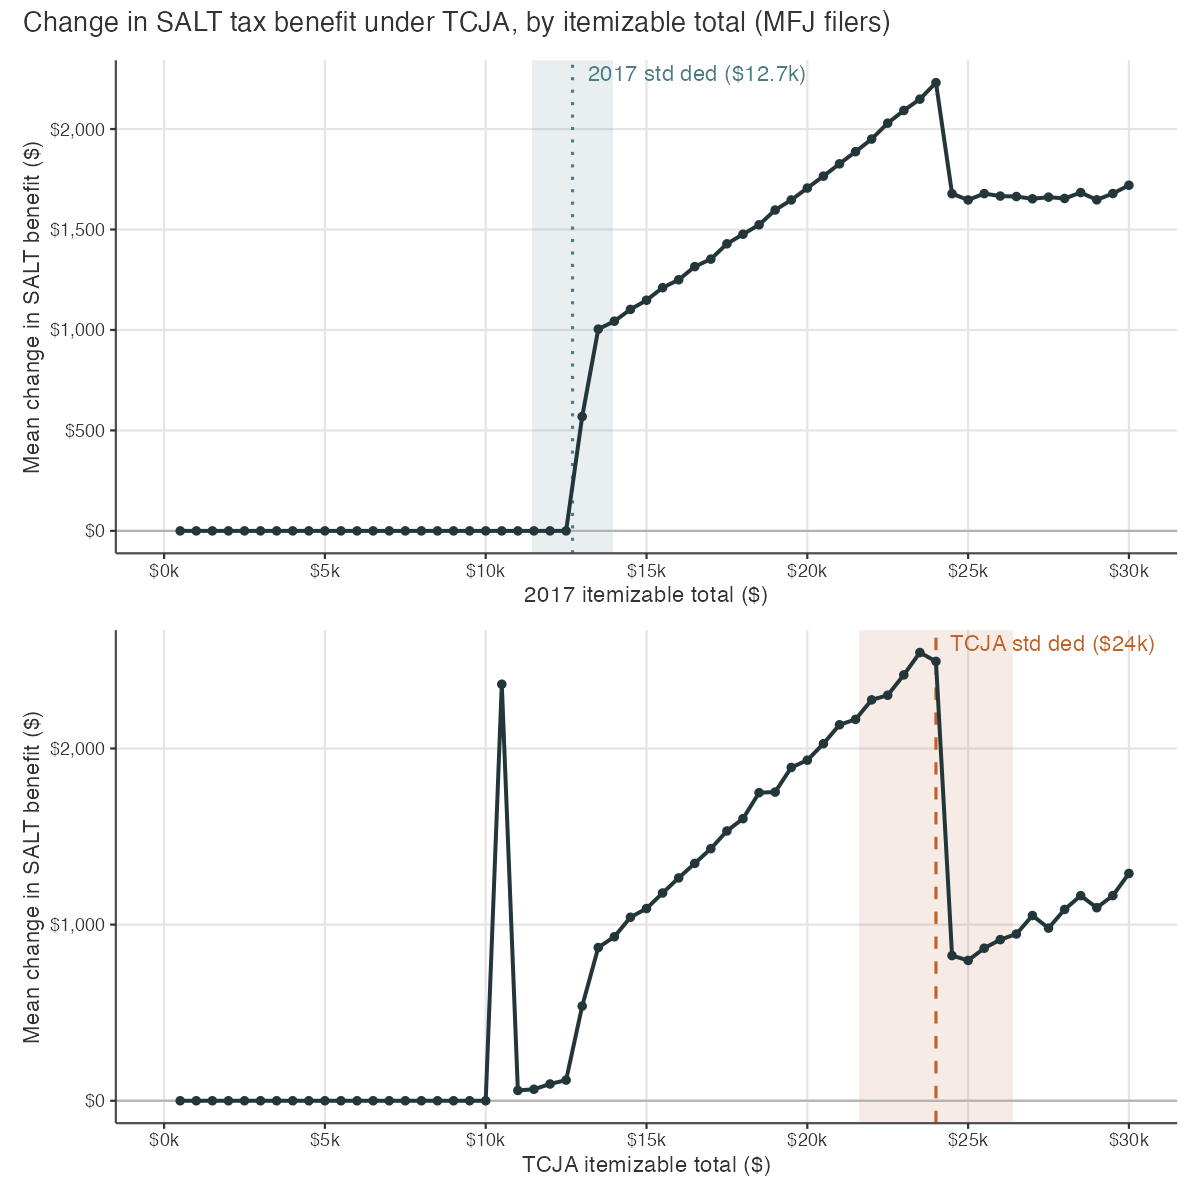
\includegraphics[width=0.78\linewidth]{10j_salt_refund_diff.png}
\caption{First stage: mean change in the SALT tax benefit under the TCJA by itemizable total, MFJ filers, \$500 bins, 2013--2023 pooled. The top panel computes the itemizable total under 2017 deduction rules; the bottom panel under TCJA rules. Shaded bands are $\pm 10\%$ windows around the 2017 (\$12.7K) and TCJA (\$24K) MFJ standard deductions.}
\label{fig:salt_refund_diff}
\end{figure}

The three groups are defined formally by imputed itemization status under the construction of Section~4: the never-itemized group has a 2017 itemizable total below the pre-TCJA standard deduction, the stopped-itemizing group falls between the pre- and post-TCJA standard deductions, and the always-itemized group lies above the post-TCJA standard deduction. Compared as whole populations, the three groups are wildly unbalanced. Table~\ref{tab:tab:balance} shows that, relative to the stopped-itemizing group, never-itemized MFJ households are six years younger and have \$72{,}000 lower income and \$6{,}000 lower SALT bills, while always-itemized households earn \$64{,}000 more, pay \$4{,}600 more in SALT, and live in \$298{,}000 more valuable homes. Within $\pm 10\%$ bands around the two standard-deduction cutoffs, however, these gaps shrink by roughly an order of magnitude: income gaps fall to \$5{,}000--15{,}000, age gaps to a fraction of a year, and SALT gaps to a few hundred to a thousand dollars. Households on either side of a cutoff are thus observably very similar, and the identifying assumption is that they are similar in unobservables as well. This motivates a difference-in-differences comparison restricted to narrow bands around each threshold; the headline specifications accordingly restrict to households whose 2017 itemizable total falls within $\pm 10\%$ of one of the two cutoffs.

\FloatBarrier
\begin{sidewaystable}

\caption{\label{tab:tab:balance}Balance table: MFJ filers. Reference group: Stopped itemizing (TCJA). OLS coefficients with standard errors in parentheses.}
\centering
\small
\setlength{\tabcolsep}{4pt}
\begin{tabular}[t]{llllll}
\toprule
Variable & \shortstack{Stopped\\(mean)} & \shortstack{Never itemized − Stopped\\(full sample)} & \shortstack{Always itemized − Stopped\\(full sample)} & \shortstack{Never itemized − Stopped\\(near \$12.7k)} & \shortstack{Always itemized − Stopped\\(near \$24k)}\\
\midrule
Age & 49.9 & 6.1 & -0.5 & 0.2 & 0.0\\
 &  & (0.0) & (0.0) & (0.0) & (0.0)\\
Household income (\$) & 152,028 & -72,274 & 64,198 & -5,371 & 14,757\\
 &  & (91.8) & (218.9) & (200.1) & (370.9)\\
Number of children & 1.12 & -0.35 & 0.13 & -0.03 & 0.02\\
\addlinespace
 &  & (0.00) & (0.00) & (0.00) & (0.00)\\
Homeowner (share) & 0.985 & -0.219 & 0.016 & -0.006 & NA\\
 &  & (0.000) & (0.000) & (0.000) & (  NA)\\
Home value, owners (\$) & 361,277 & -142,863 & 298,482 & -20,432 & 65,199\\
 &  & (279.9) & (751.2) & (700.4) & (1,165.0)\\
\addlinespace
Total SALT (\$) & 8,695 & -6,053 & 4,573 & -438 & 1,053\\
 &  & (5.1) & (12.9) & (8.9) & (21.3)\\
Marginal federal tax rate & 0.183 & -0.114 & 0.032 & -0.006 & 0.005\\
 &  & (0.000) & (0.000) & (0.000) & (0.000)\\
Metropolitan area (share) & 0.847 & -0.076 & -0.011 & -0.008 & -0.006\\
\addlinespace
 &  & (0.000) & (0.001) & (0.001) & (0.001)\\
Pre-TCJA move rate & 0.059 & 0.030 & 0.007 & -0.000 & 0.004\\
 &  & (0.000) & (0.001) & (0.001) & (0.001)\\
\bottomrule
\end{tabular}
\end{sidewaystable}


The estimating equation is a standard group-specific event study,
\[
y_{ist} \;=\; \sum_{k \ne 2017} \beta_k \cdot \mathbbm{1}[t = k] \cdot G_i \;+\; X_{it}' \gamma \;+\; \mu_{st} \;+\; \varepsilon_{ist},
\]
where $y_{ist} = \mathbbm{1}[\text{household } i \text{ moved in year } t]$ is the ACS one-year mover indicator, $G_i$ is an indicator for the treatment group (always-itemized or stopped-itemizing, with the never-itemized control omitted), and $X_{it}$ collects controls for age, marital status, sex of the household head, and education. The fixed effect $\mu_{st}$ is a state-by-year fixed effect that absorbs any time-varying state-level shock common to all households in a given state and year, and standard errors are clustered by state.

Identification rests on parallel trends conditional on exposure group and the observable controls. The credibility check is whether pre-2017 trajectories of within-group moving rates are flat after this conditioning. In the raw data the three groups have visibly divergent levels and pre-trends -- always-itemized households were on a clearly rising trajectory before 2017 -- so the conditional event study is what the design depends on.

\subsection*{Results}

\begin{figure}[h!]
\centering
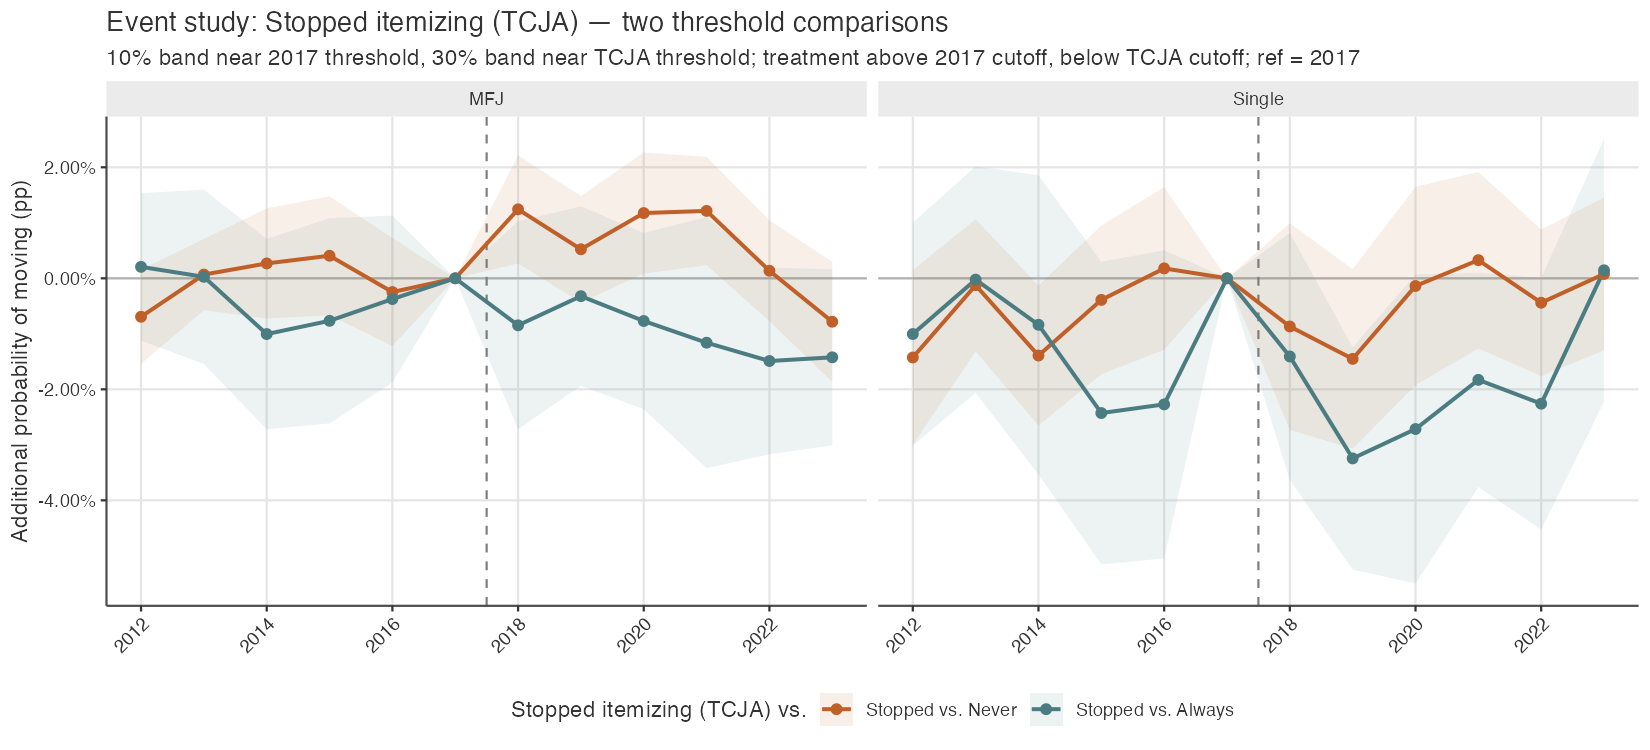
\includegraphics[width=\linewidth]{10b_event_study.png}
\caption{Conditional event study: moving rates by itemization group and filing status, $\pm 10\%$ window around each 2017 standard-deduction cutoff; reference year 2017; controls and state-by-year fixed effects; standard errors clustered by state.}
\label{fig:event_study}
\end{figure}

Figure~\ref{fig:event_study} reports the conditional event-study coefficients by filing status. For MFJ filers the post-2017 coefficients on both treatment groups are statistically and economically indistinguishable from zero -- a clear null on the extensive margin. For single filers there is some evidence of a positive post-2017 effect, concentrated in the stopped-itemizing group at the lower (\$12.7K) standard-deduction cutoff, where the SALT-cap-induced change in the effective local tax rate is largest in proportional terms.

Pooled point estimates of the post-2017 treatment effect span $-0.5$ to $+0.5$ percentage points across the four combinations of treatment group (always-itemized, stopped-itemizing) and filing status (MFJ, single), against a baseline annual moving rate between 6 and 8 percent. This corresponds to a $-10$ to $+10$ percent change in the moving rate relative to baseline. The corresponding change in the effective local tax price for affected itemizers is $1/(1-T'(y))$ times the pre-TCJA price, where $T'(y)$ is the household's marginal federal income tax rate. Dividing the relative moving-rate response by the relative tax-price increase yields implied extensive-margin migration elasticities of $-0.5$, $-0.3$, $+0.2$, and $+0.5$ across the four configurations. The estimates straddle zero and no sign is consistent across treatment groups or filing statuses, which is the basis for reading the extensive-margin evidence as a null. These magnitudes are substantially below the high-income migration elasticities found in some of the existing literature \citep{drukker, AkcigitBaslandzeStantcheva2016} and below some of the calibrated values used in recent quantitative spatial work on local labor markets and migration \citep{SprungKeyserHendrenPorter2024}.

A complementary look at the intensive margin asks where exposed households move conditional on moving. For each mover I compute the SALT bill that the household would face if it retained its origin-PUMA income and home value but lived in the destination PUMA, and compare it to the SALT bill at the origin PUMA. Figure~\ref{fig:cond_mig_salt} reports the difference (destination minus origin) in event-study form, by filing status and treatment group. Pre-2017 differences are near zero. Post-2017, stopped-itemizing movers consistently relocate to PUMAs where the imputed SALT bill at constant household characteristics is several hundred to one thousand dollars \emph{higher} than at their origin, in both MFJ and single filers. Always-itemized movers show no comparable pattern. This is the opposite of what a pure tax-avoidance migration story would predict; I do not yet have a clean explanation for it.

\begin{figure}[h!]
\centering
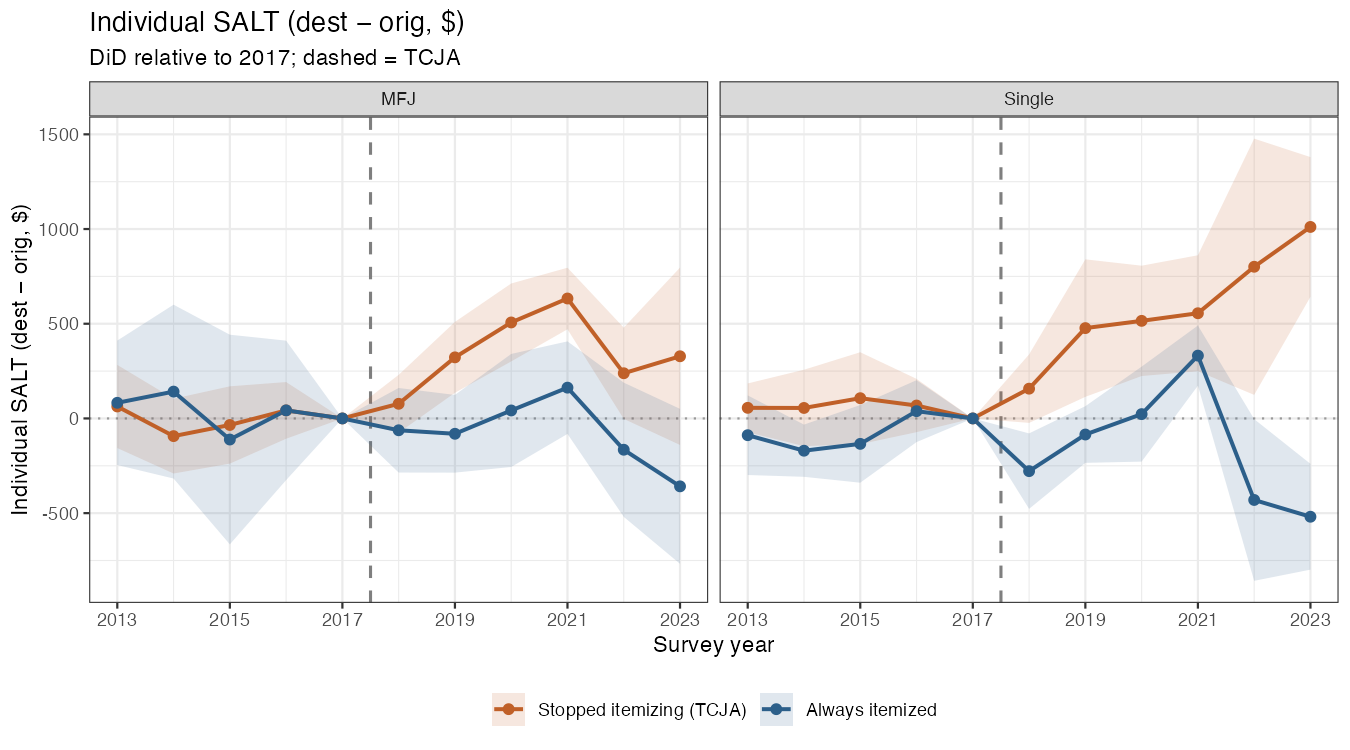
\includegraphics[width=\linewidth]{cond_mig_es_salt_diff.png}
\caption{Conditional on moving, difference between destination-PUMA and origin-PUMA SALT bills evaluated at fixed origin household characteristics. Event-study coefficients relative to 2017, by filing status and treatment group. Dashed line marks TCJA.}
\label{fig:cond_mig_salt}
\end{figure}

\subsection*{Heterogeneity and Robustness}

Heterogeneity in the treatment effect, reported in Appendix~B, is limited: across age, education, presence of children, metropolitan status, multigenerational living arrangements, race, and sex of the household head, the response is qualitatively similar.

The design has two limitations that deserve explicit acknowledgment. The first is the imputation error in group assignment. The one-sided measurement error documented in Section~4 means that true itemizers can leak into the never-itemized control group, biasing the estimated treatment effects toward zero. One way of addressing this is to shift the range of control households further toward those with lower imputed itemizable totals -- households well below the standard deduction are very unlikely to be misclassified, since the upward-biased imputation would have to be implausibly large to push them above the cutoff. The cost of this tightening is that those households make worse controls along observables, since they sit further from the treated groups in the income distribution. I have run this exercise and the results look qualitatively similar to the headline specifications. The second limitation is the state PTET workarounds, which attenuate the true treatment difference between cap-bound and unaffected itemizers in NY, CA, NJ, CT, and a handful of others post-2021. I plan to address this by subsetting the sample to non-PTET states.


\section{Local Government Revenue Responses}

The county-revenue design treats county-level SALT-cap exposure as a continuous, place-specific treatment intensity. As described in Section~4, exposure is the mechanical 2017--2018 change in effective SALT per filer in each county, constructed from IRS SOI returns. Counties with many cap-bound or formerly-itemizing filers have high exposure; counties dominated by never-itemizers have exposure close to zero. The cross-county distribution of exposure has substantial mass in the right tail, and that variation -- across all counties, not just those at the extremes -- is the source of identification.

The estimating equation interacts exposure with year fixed effects,
\[
\log y_{it} \;=\; \alpha_i + \beta_t + \sum_{k \ne 2017} \theta_k \cdot \mathbbm{1}[t = k] \cdot \text{Exposure}_i \;+\; \varepsilon_{it},
\]
where $y_{it}$ is local revenue for county $i$ in year $t$. I estimate the equation separately for total tax revenue, property tax revenue, federal intergovernmental transfers, and state intergovernmental transfers. The model includes county fixed effects $\alpha_i$ and year fixed effects $\beta_t$; the headline specification additionally absorbs state-by-year shocks via $\beta_{s(i)t}$, which controls for any state-level confounder that moves all counties within a state in the same year. Standard errors are clustered at the state level throughout.

Identification rests on the assumption that, conditional on county fixed effects, common time shocks, and (in the headline specification) state-by-year shocks, exposure intensity is uncorrelated with other determinants of revenue trends -- the ``strong'' parallel-trends condition for continuous treatments studied by \cite{CallawayGoodman-BaconSantanna2024}. This is a substantive assumption. The TCJA contained many provisions other than the SALT cap (a corporate rate cut, expensing changes, child tax credit reforms), and several of these are correlated with high-SALT geographies. Decomposing the revenue response by source partially mitigates this concern: the property-tax channel is most directly tied to local migration and assessed-value adjustments, while federal intergovernmental transfers are likely contaminated by unrelated federal policy, in particular the CARES Act and the American Rescue Plan. I therefore treat the federal-IG response as a falsification check rather than as a primary outcome.

Figure~\ref{fig:revenue_total} shows the event-study coefficients $\theta_k$ on Exposure $\times$ year for log total local tax revenue, under the headline specification with state-by-year fixed effects. The pre-2017 coefficients are essentially flat and statistically indistinguishable from zero. From 2018 onward, the coefficient turns negative and trends downward, reaching statistical significance at the five-percent level by 2020 and remaining significant through 2022. The post-period dynamic is steady rather than abrupt, consistent with a mechanism that operates through gradual migration-driven adjustment of the local tax base rather than a one-time discrete shift.

\begin{figure}[h!]
\centering
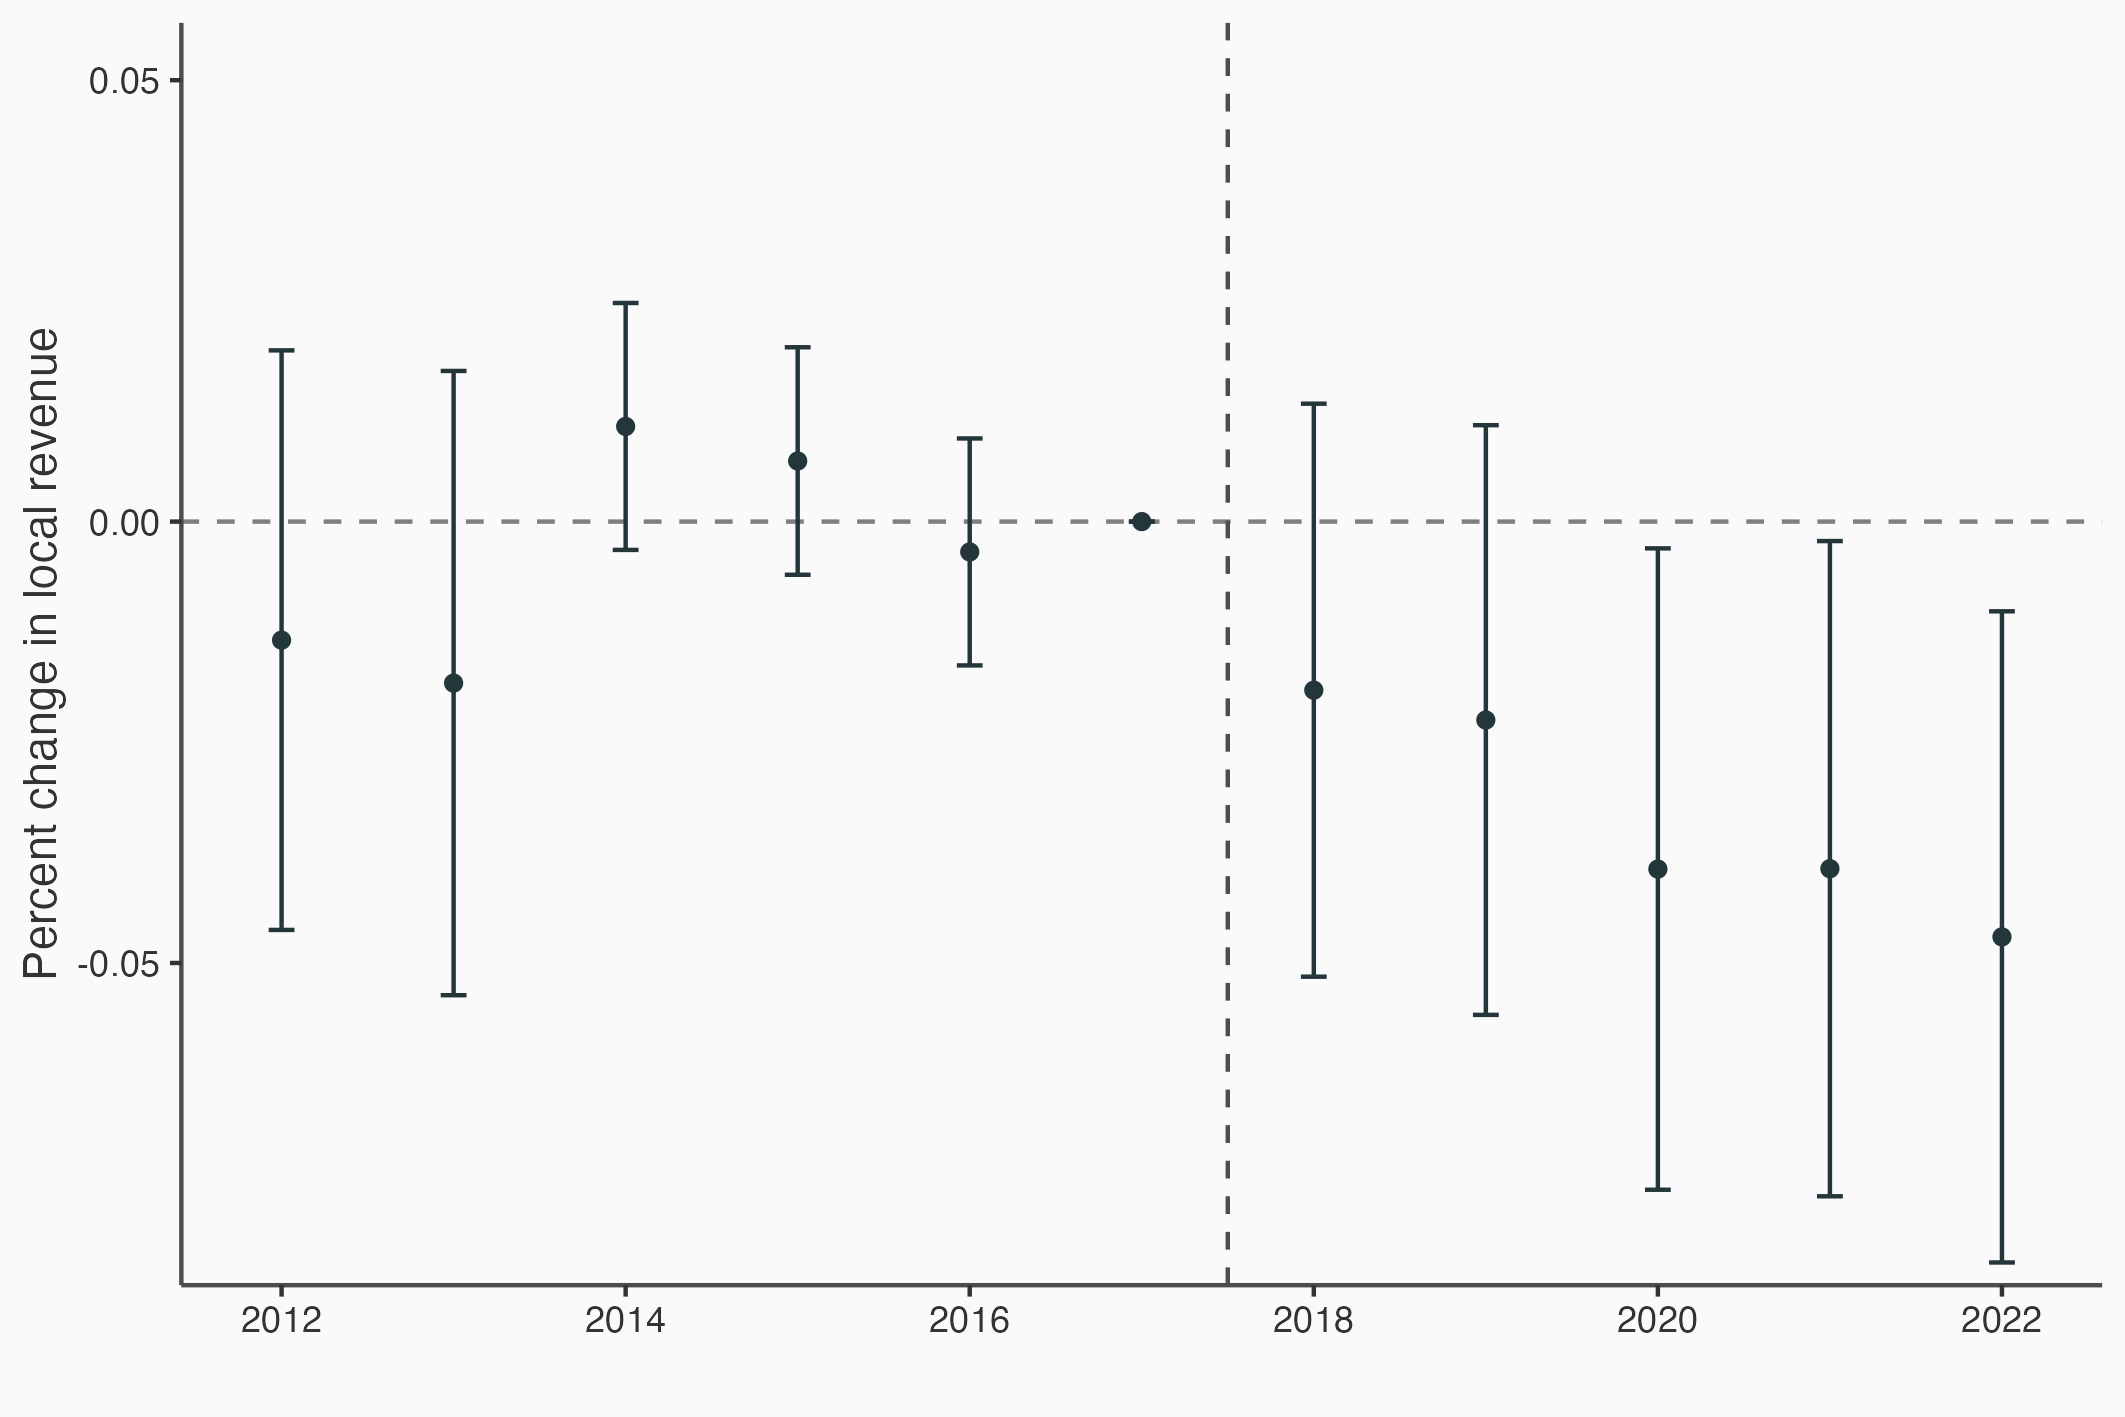
\includegraphics[width=0.78\linewidth]{fig_effective_salt_year_interactions_total_tax.png}
\caption{County-level event study: log total local tax revenue regressed on county exposure interacted with year fixed effects, with county and state-by-year fixed effects. Reference year 2017. Standard errors clustered at the state level.}
\label{fig:revenue_total}
\end{figure}

Figure~\ref{fig:revenue_sources} shows the decomposition by revenue source. Property tax revenue declines modestly and statistically significantly in the immediate post-2018 years; this pattern is consistent with the migration discussion in Section~5, since out-migration of high-bracket households reduces assessed values and property reassessment cycles are short enough for revenue to respond in the same window. Federal intergovernmental revenue declines sharply but noisily, with a particularly large negative coefficient in 2021; this response is likely contaminated by CARES Act and ARP allocations that were correlated with state and local characteristics other than SALT exposure, and I do not interpret it causally. State intergovernmental revenue is roughly flat throughout the post-period, with weak evidence of decline in 2018--2019 and at the end of the panel.

\begin{figure}[h!]
\centering
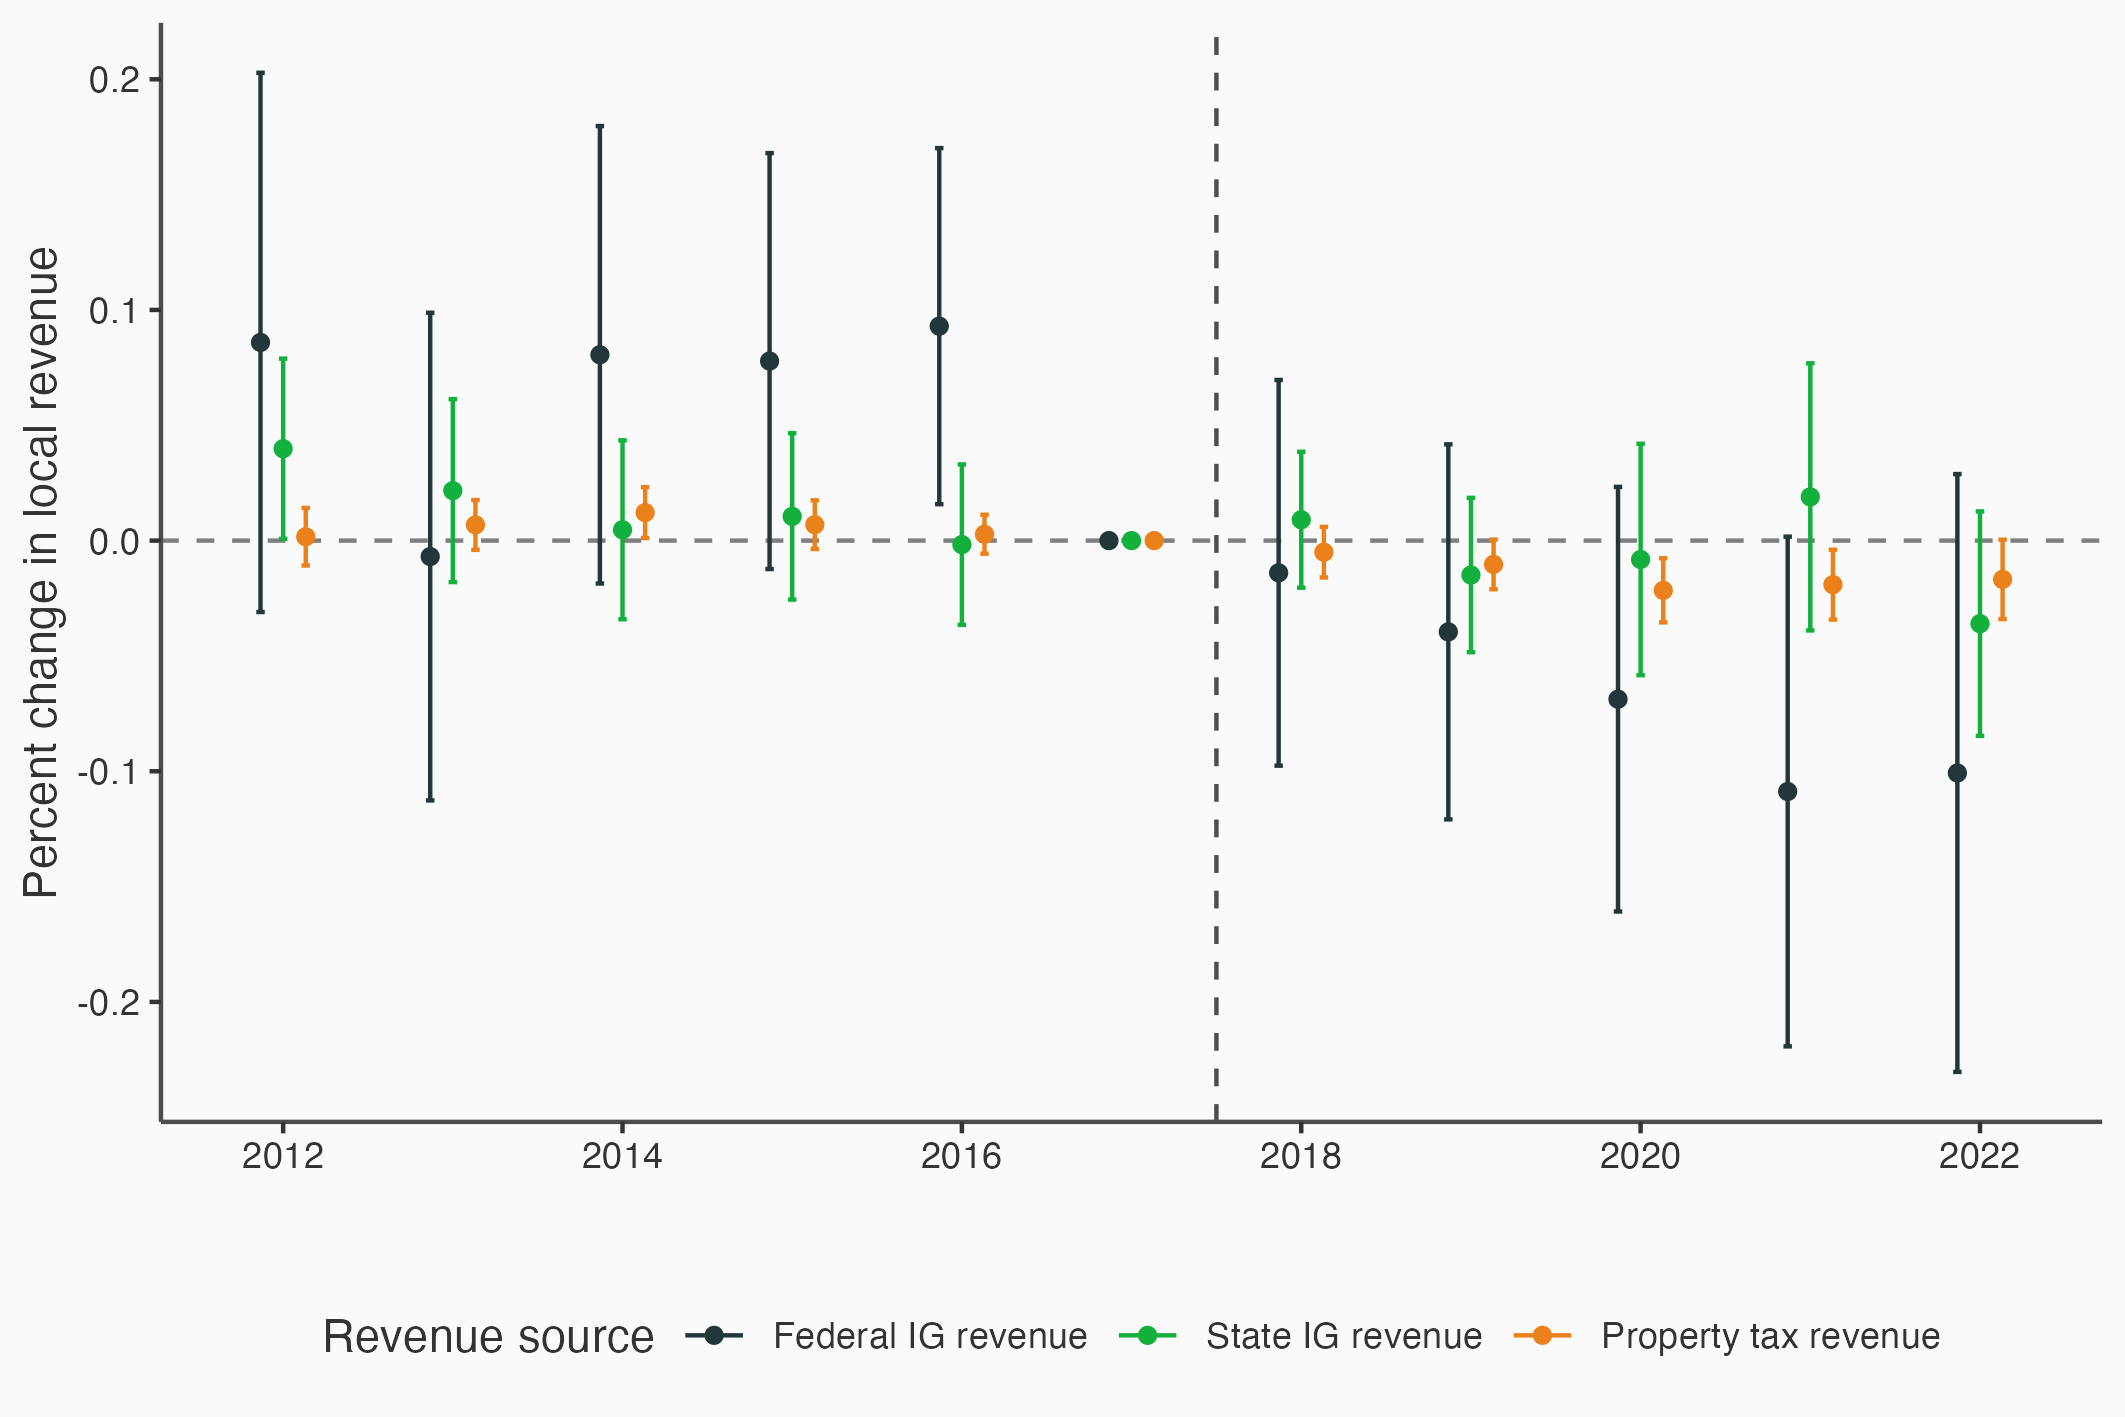
\includegraphics[width=0.85\linewidth]{fig_effective_salt_year_interactions_revenue_sources.png}
\caption{County-level event study by revenue source: federal intergovernmental, state intergovernmental, and property tax revenues, regressed on county exposure interacted with year fixed effects.}
\label{fig:revenue_sources}
\end{figure}

A causal interpretation of the total-revenue response requires the assumption that other TCJA provisions are not driving the pattern, which is difficult to defend in isolation. The property-tax response is more directly tied to the migration evidence in Section~5: the property-tax base is the channel through which household-level migration most plausibly translates into local revenue, and the response is small, precisely estimated, and contemporaneous with the migration response. The magnitude of the federal-IG response indicates that contemporaneous federal-policy variation is large relative to any SALT-cap signal in that revenue source.

The revenue design has four limitations that mirror those of the migration design and that the planned robustness work will address. First, other TCJA provisions are spatially correlated with SALT exposure and could in principle confound the total-revenue effect; the source decomposition partially addresses this. Second, the exposure measure is constructed from the mechanical 2017--2018 change and does not adjust for the subsequent rollout of pass-through-entity workarounds, so true post-2021 exposure is overstated in NY, CA, NJ, CT, IL, and MA; I will re-estimate after dropping these states and construct alternative exposure measures that exclude pass-through-eligible filers. Third, the Census Annual Survey of Local Government Finances is sample-based in non-Census years, making annual variation noisier than the five-year census waves; I will report robustness restricting estimation to the five-year census waves. Fourth, the federal-IG response is large but almost certainly the wrong window onto the SALT cap's causal effect given the coincidence with pandemic-era federal transfers, and it should be treated as a check rather than a primary outcome.

Both research designs rely on public-use data. Identification holds under standard checks in both cases but remains uncertain along three dimensions: group-classification noise in the ACS, confounding from contemporaneous federal policy in the revenue regression, and PTET workarounds in both designs. The two designs imply that out-migration of exposed households should erode the property-tax base in exposed jurisdictions; the qualitative magnitudes are broadly consistent with this prediction.


\section{Conceptual Framework}

This section provides a brief and incomplete sketch of the discrete-choice spatial-equilibrium model that will eventually be used to interpret the reduced-form estimates and to construct counterfactuals. The model is not yet estimated.

A metropolitan area is populated by a unit mass of households indexed by $i$ with income $Y_i$ and a vector of observable demographics $z_i$ (age, household composition, education), drawn from a joint distribution $F(Y, z)$. Each household chooses one of $J$ jurisdictions in which to reside. Following the recent quantitative spatial literature, per-household housing demand is inelastic at one unit; each resident of jurisdiction $j$ pays the gross rental rate $p_j$ and consumes the residual income as numeraire $x_i$. Indirect utility from residing in $j$ is log-additive,
\[
V_{ij} \;=\; \alpha(z_i) \log g_j \;+\; \gamma(z_i) \log \!\left[Y_i - p_j\right] \;+\; \xi_j \;+\; \varepsilon_{ij}, \quad \varepsilon_{ij} \sim \text{Gumbel}(\theta),
\]
where $g_j$ is per-household local public-good provision, $\xi_j$ is an unobserved jurisdiction amenity, $\theta$ is the Gumbel scale parameter governing the variance of taste shocks, and $\alpha(z_i)$, $\gamma(z_i)$ are demographic-shifted taste coefficients. The Gumbel assumption delivers closed-form logit choice probabilities, which is what makes the model tractable for estimation and counterfactual analysis.

Housing is supplied by a constant-elasticity production technology in each jurisdiction,
\[
\log H_s^j(p_s^j) \;=\; \lambda + \eta \log p_s^j + B_j,
\]
where $\eta$ is the housing supply elasticity and $B_j$ is a jurisdiction-specific productivity shifter capturing geography, regulation, and local construction technology. Suppliers receive the net-of-tax price $p_s^j$ while households pay the gross price $p_j = (1 + t_j)\, p_s^j$, where $t_j$ is the property tax rate. Under full congestion of the local public good and jurisdictional budget balance, per-household public-good provision satisfies $g_j = t_j\, p_s^j = p_j - p_s^j$ -- the property-tax wedge is precisely the per-household level of public-good provision.

Given an exogenous vector of property tax rates $\mathbf{t}$, an equilibrium consists of supplier prices, gross prices, public-good levels, populations, and household choice probabilities such that the price relationship, household optimality, housing-market clearing, and jurisdictional budget balance all hold simultaneously in every jurisdiction. The four conditions jointly determine the equilibrium as a fixed point: choice probabilities depend on $(p_j, g_j)$ through indirect utility, populations $N_j$ aggregate those probabilities, supplier prices clear the housing market at each $N_j$, and budget balance closes the system.

The SALT cap operates in the model as a shock to the effective tax rate faced by itemizing households. Before TCJA, the federal SALT deduction effectively scaled each itemizing household's local tax rate by $(1 - T'(Y_i))$; the cap raises the effective $t_j$ faced by cap-bound itemizers back toward the statutory rate. Three first-order effects follow. The gross rental rate $p_j$ rises for exposed households, lowering their indirect utility from residing in $j$. This lowers the logit choice probability for $j$ among exposed households, generating out-migration -- the channel identified in Section~5. The change in $N_j$ then shifts the budget-balance condition, with the sign of the effect on $g_j$ depending on whether jurisdictions hold $t^{\text{stat}}_j$ fixed and let revenue fall, or raise it to defend the public-good level. The reduced-form estimates of Section~6 -- modest revenue declines but no detectable rise in tax rates -- suggest the former dominates in the short run.

This mapping between model and empirics is what makes the proposal's structural ambition feasible. The migration coefficient from Section~5 maps to the slope of the logit choice probability evaluated at the indifference margin, identifying a combination of $\theta$ and the spatial gradient of $\alpha(z) \log g_j - \gamma(z) \log[Y_i - p_j]$. The revenue coefficient from Section~6 maps to the partial derivative of $N_j$ with respect to $t_j$ multiplied by the share of exposed filers and baseline SALT per filer, plus any adjustment in $t^{\text{stat}}_j$ that jurisdictions undertake. Combined with additional moments on rents, prices, and the directions of observed moves, the two coefficients move the model toward identification of the Gumbel scale parameter $\theta$, the housing supply elasticity $\eta$, and the average taste-for-public-goods parameter $\bar\alpha$.

The workhorse model has three caveats worth flagging up front, each of which the structural extension will address. First, inelastic housing demand at $h_i = 1$ implies that the property tax functions effectively as a poll tax on residents of $j$, with no within-jurisdiction free-riding inefficiency for a federal SALT subsidy to compensate for. This is a substantive limitation of the workhorse model, and optimal-policy statements from it should be qualified accordingly; the natural extension is to add elastic $h_i$ through a CES inner nest. Second, the tax incidence in the workhorse model falls fully on landowners, since supply is upward-sloping but demand is inelastic. Distributional conclusions therefore depend on landowner identity, which the proposal does not currently model; the structural extension will integrate this margin. Third, the model contains no political-economy channel through which jurisdictions adjust $t^{\text{stat}}_j$ in response to revenue shocks. The reduced-form evidence does not suggest sharp rate-side responses in the post-TCJA window -- jurisdictions appear to have let revenue fall rather than raise rates -- but a structural extension will embed a median-voter or local-political-economy step to make this margin endogenous rather than assumed away.


\section{Discussion, Open Questions, and Path Forward}

Three limitations of the analysis as it stands suggest natural next steps.

The first is statistical power. The ACS public-use sample is large in absolute terms but thin once restricted to the narrow itemizable-total bands around the standard-deduction cutoffs, and the confidence intervals on the estimated migration elasticities are correspondingly wide. Extending the analysis to additional data sources would help. Infutor provides individual-level move histories at higher frequency than the ACS, CoreLogic provides homeownership and property-transaction records, and Data Axle provides income and demographic information; together these would allow the migration design to be re-estimated on a much larger and more longitudinally detailed sample.

The second is that the model in Section~7 is incomplete. The natural next step is a first pass at estimating the discrete-choice spatial-equilibrium model on the reduced-form moments documented here, even in a stylized form. This would discipline the interpretation of the elasticities, generate quantitative predictions for the speed-of-adjustment and incidence questions raised in the introduction, and identify which additional moments are most useful to bring in.

The third is mechanism. The property-tax-revenue decline in Section~6 is consistent with the migration channel, but it is also consistent with two alternative mechanisms that the current design cannot separate: a mechanical decline in assessed property values in exposed jurisdictions, or a political-economy response in which voters in exposed jurisdictions become less willing to approve property-tax increases. The school-bond referendum data assembled by \cite{BiasiLafortuneSchonholzer2025} provides a direct measure of the latter -- approval rates for local school-capital referenda across 29 U.S. states with staggered timing -- and merging it to the county-level SALT exposure measure would allow a test of whether the revenue decline operates through political resistance or only through the mechanical channel.

\bibliography{sample}


\appendix
\section{ACS Itemization Imputation: Validation}

This appendix benchmarks the ACS-imputed household itemization status against the actual IRS-published itemization rates from SOI returns, using the validation pipeline in\\\texttt{code/analysis/returns/validate\_itemization.R}.

Figure~\ref{fig:validate} compares the weighted-average national itemization rate over time (left panel) and at the state-year level (right panel), in each case computed from the ACS using the imputed household-level itemization indicator and from the IRS SOI using the published count of returns with itemized deductions. Both series fall sharply at TCJA in 2017--2018, consistent with the institutional change. The ACS-imputed rate sits systematically below the SOI rate by a level shift that is roughly stable across years and across states; this is exactly the pattern predicted by the one-sided measurement error documented in Section~4, since the imputed itemizable total is a lower bound on the truth and the imputed itemization indicator is therefore an under-classification. State-level points in the right panel cluster tightly along a line parallel to the 45$^\circ$, again consistent with a roughly state-uniform downward shift rather than state-specific imputation failures.

\begin{figure}[h!]
\centering
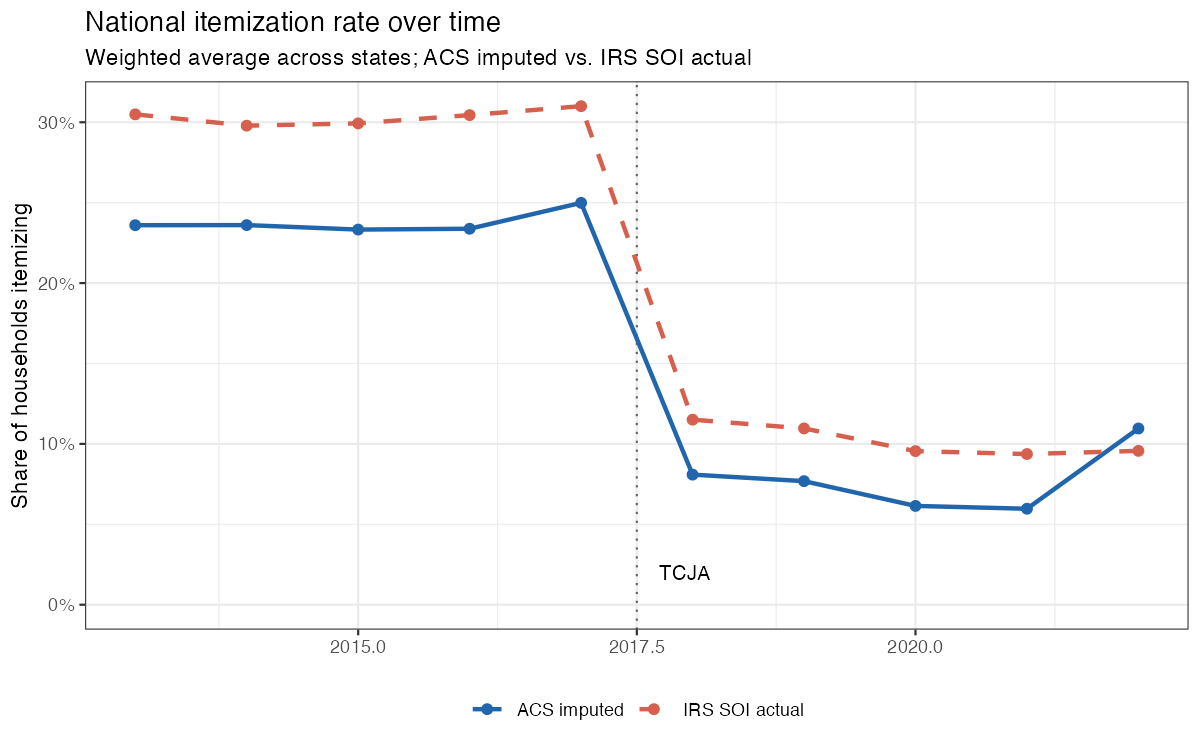
\includegraphics[width=0.48\linewidth]{validate_itemize_time.png}
\hfill
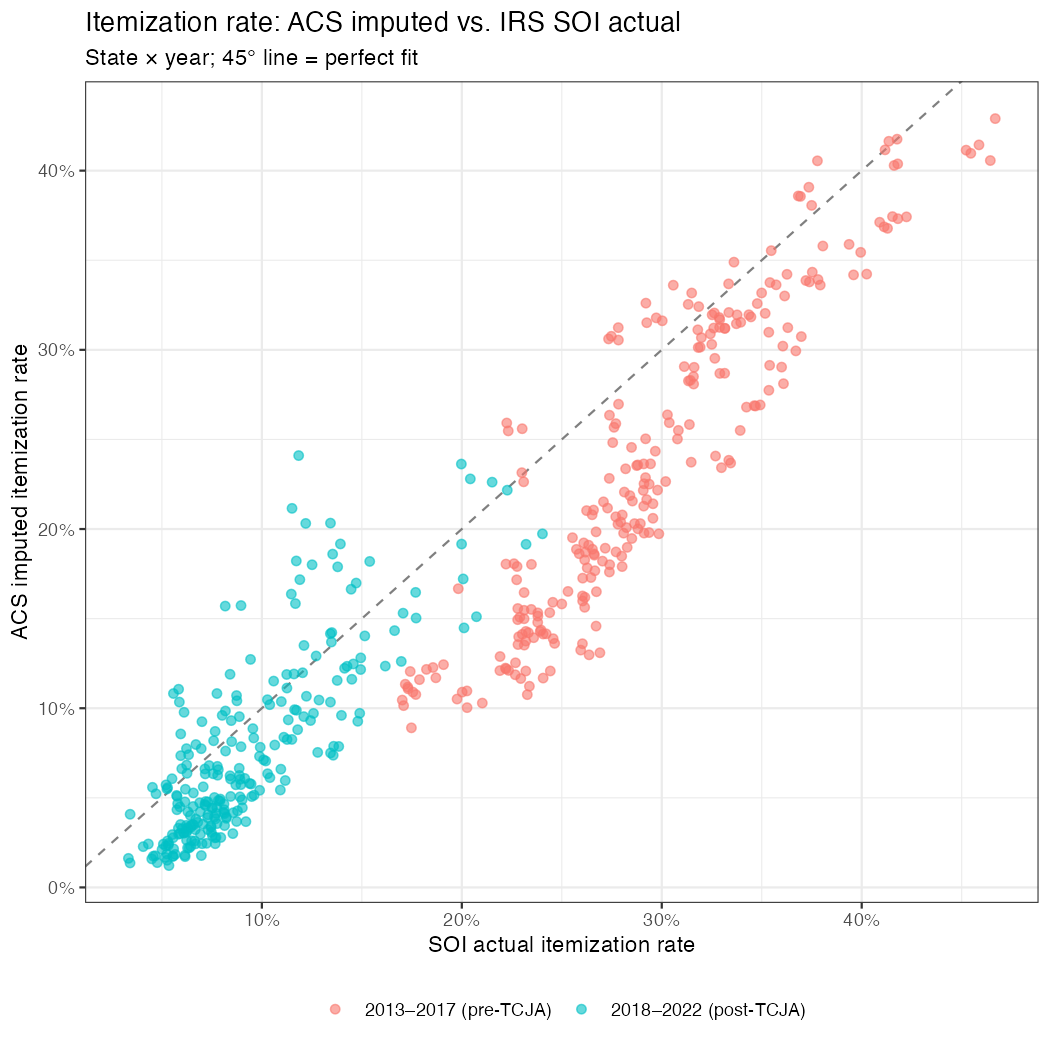
\includegraphics[width=0.48\linewidth]{validate_itemize_state.png}
\caption{Validation of ACS itemization imputation. Left: national itemization rate over time, ACS imputed vs. IRS SOI actual; weighted average across states; vertical dotted line marks TCJA. Right: state $\times$ year scatter, ACS-imputed vs. IRS SOI-actual rate; dashed line is 45$^\circ$.}
\label{fig:validate}
\end{figure}

Quantitatively, the state-level Pearson correlation between ACS-imputed and SOI-actual rates is $0.91$ pre-TCJA ($R^2 = 0.84$) and $0.81$ post-TCJA ($R^2 = 0.66$). The mean ACS-imputed itemization rate is $23.5\%$ pre-TCJA versus $29.2\%$ in SOI, and $7.5\%$ post-TCJA versus $9.2\%$ in SOI; the imputation underestimates the rate by roughly five to six percentage points in both periods, consistent with a stable one-sided level shift rather than a TCJA-induced break. The county-level correlations tell the same story ($0.94$ pre, $0.83$ post; $R^2 = 0.88$ and $0.68$). The key implication for the migration design is that imputation noise is plausibly close to additive at the state level, supporting the conservative-bias argument of Section~4.


\section{Heterogeneity in the Migration Response}
\label{app:heterogeneity}

This appendix reports treatment-effect heterogeneity in the always-itemized event-study coefficients across seven demographic splits. Across all dimensions, the response is qualitatively similar -- there is little evidence that any one demographic group drives the headline pattern.

\begin{figure}[h!]
\centering
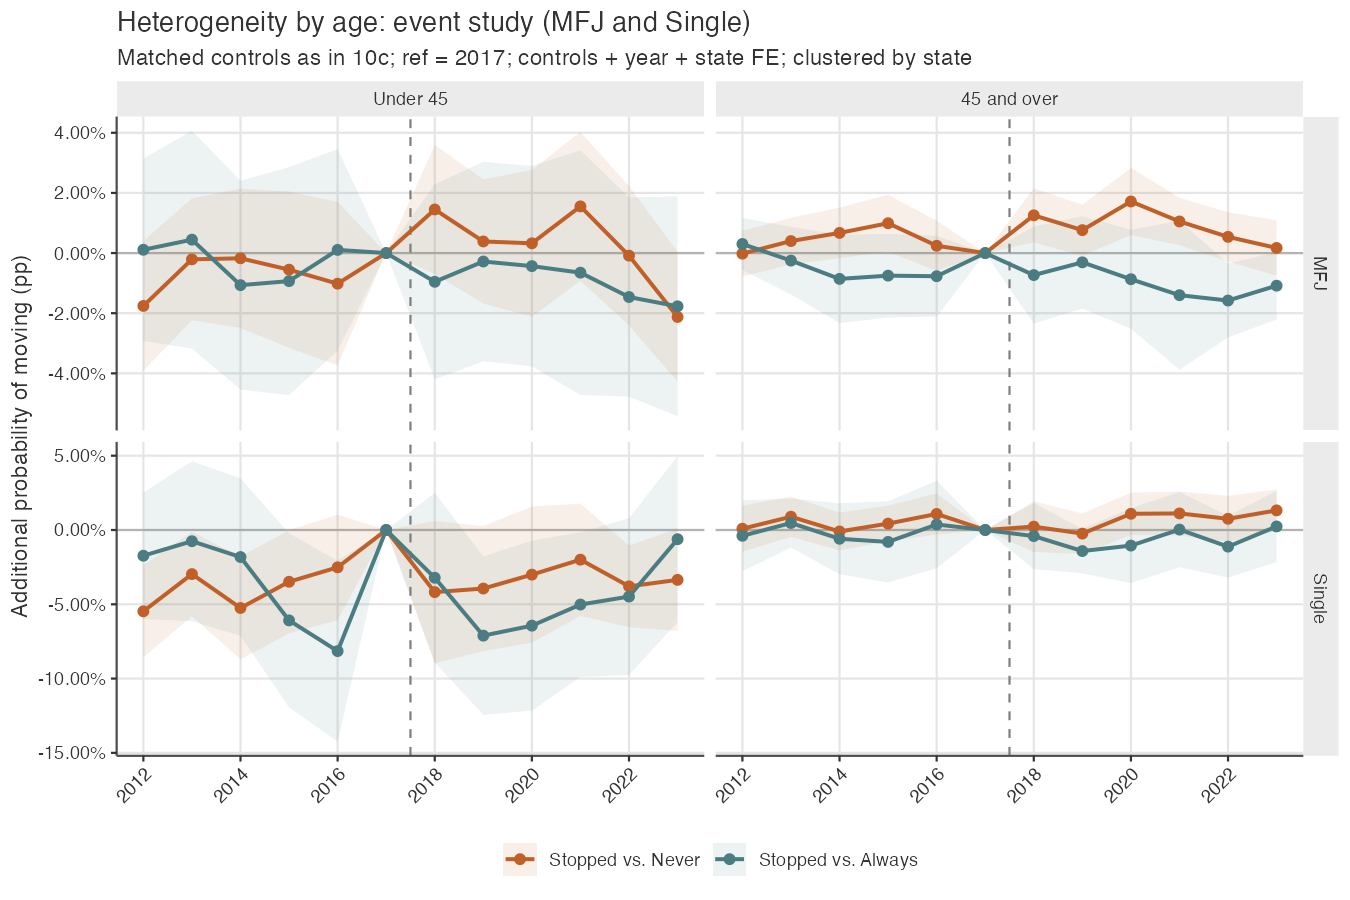
\includegraphics[width=0.7\linewidth]{10d_het_age.png}
\caption{Heterogeneity by age of household head.}
\end{figure}

\begin{figure}[h!]
\centering
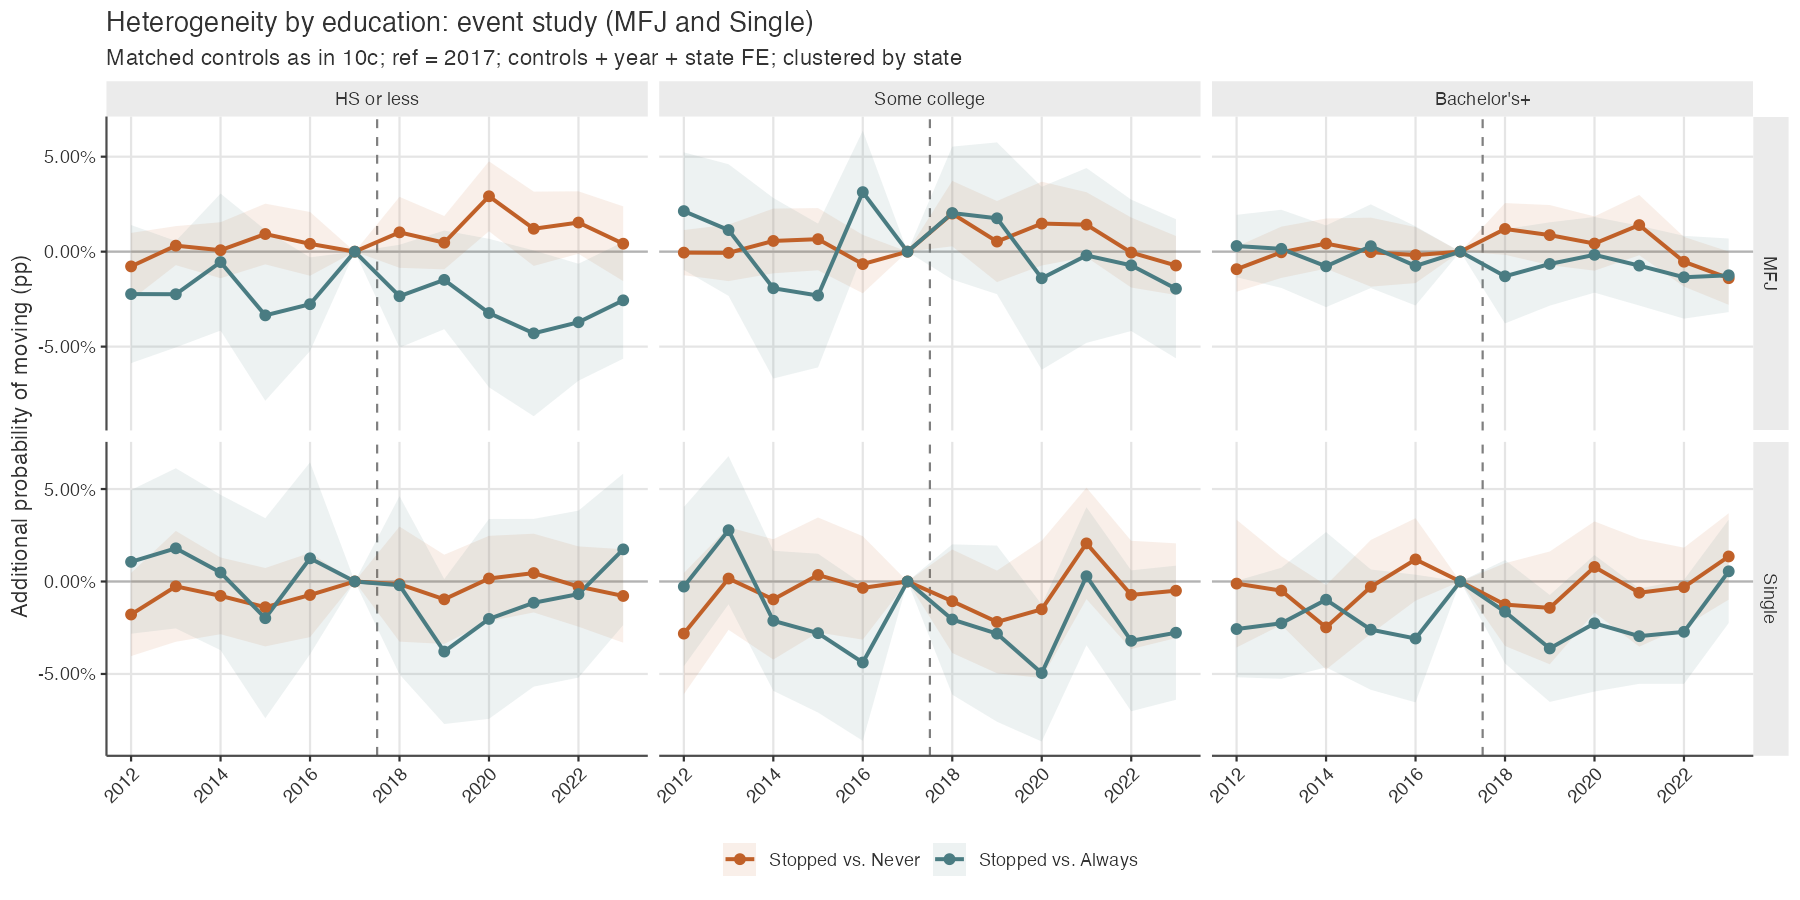
\includegraphics[width=0.7\linewidth]{10d_het_education.png}
\caption{Heterogeneity by education of household head.}
\end{figure}

\begin{figure}[h!]
\centering
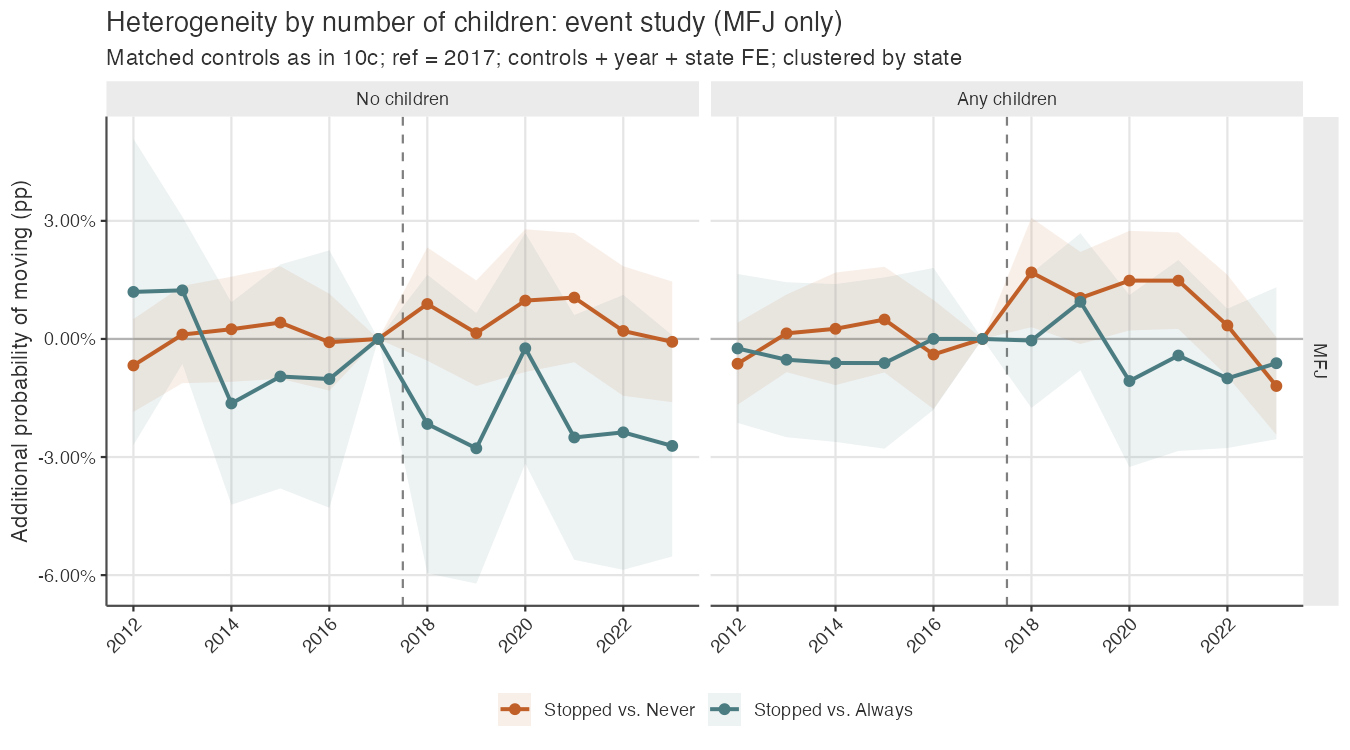
\includegraphics[width=0.7\linewidth]{10d_het_children.png}
\caption{Heterogeneity by presence of children in the household.}
\end{figure}

\begin{figure}[h!]
\centering
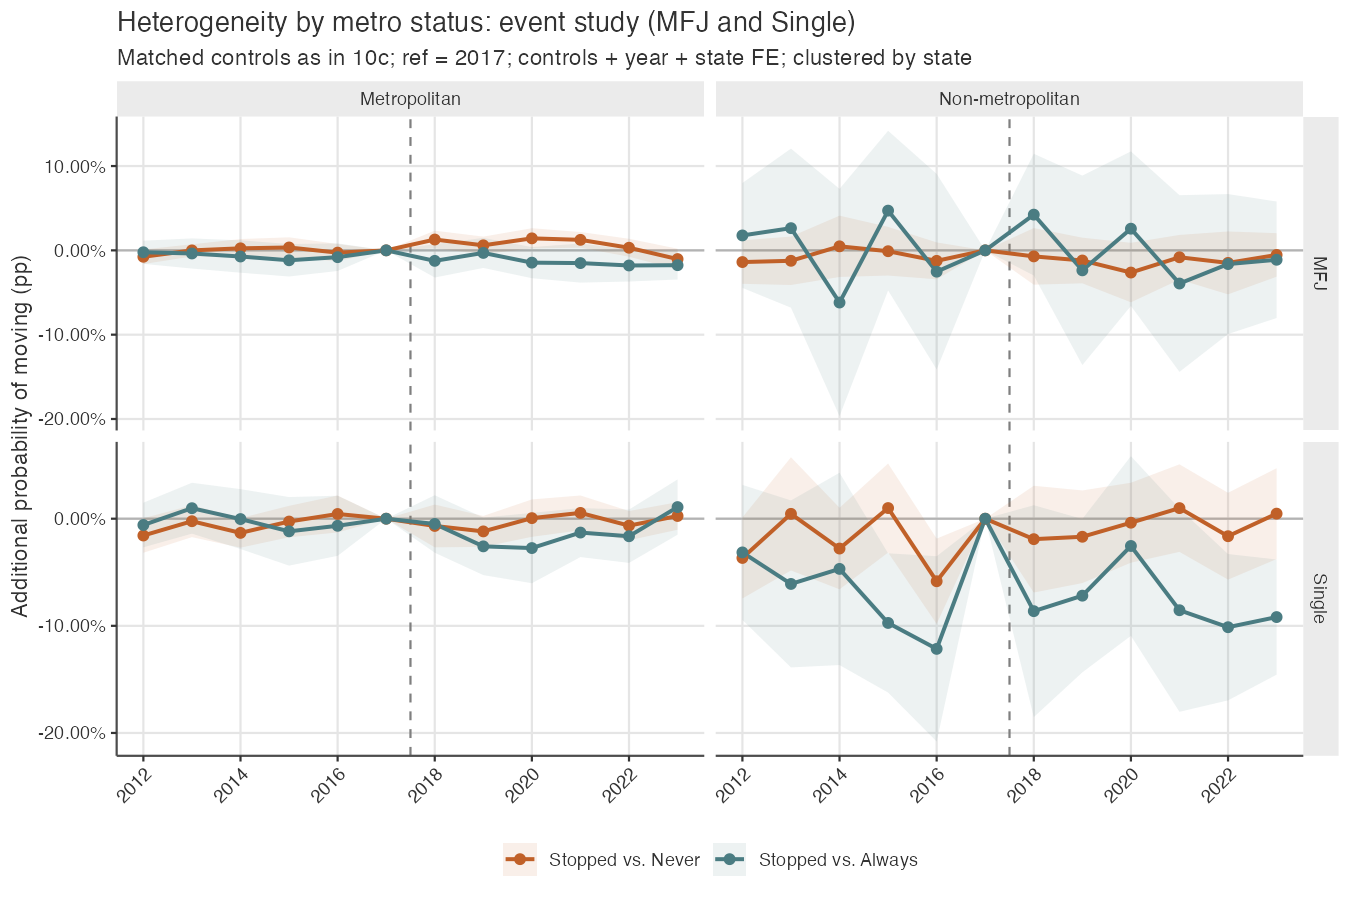
\includegraphics[width=0.7\linewidth]{10d_het_metro.png}
\caption{Heterogeneity by metropolitan vs. non-metropolitan residence.}
\end{figure}

\begin{figure}[h!]
\centering
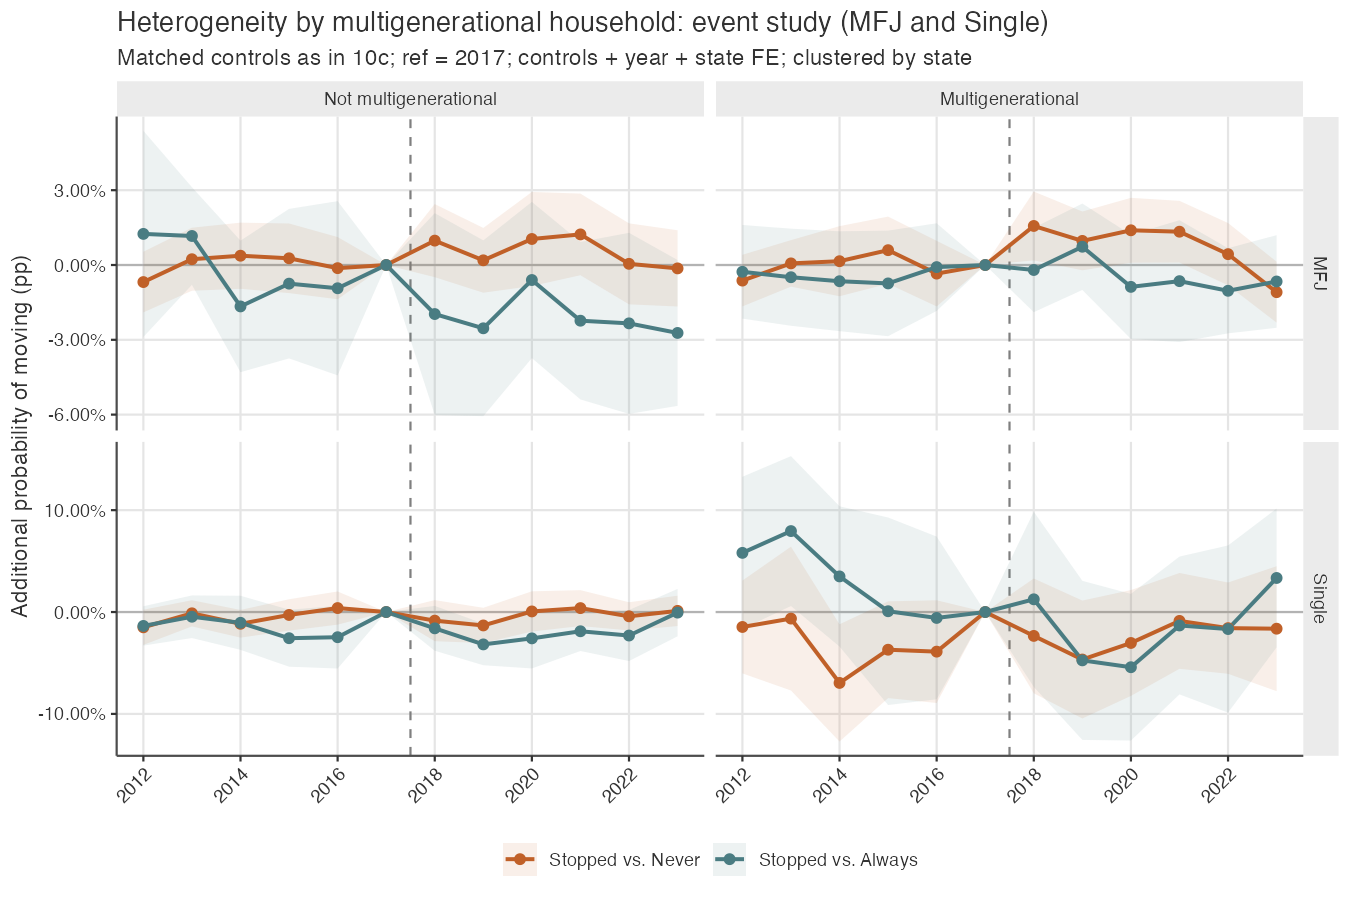
\includegraphics[width=0.7\linewidth]{10d_het_multigen.png}
\caption{Heterogeneity by multigenerational living arrangement.}
\end{figure}

\begin{figure}[h!]
\centering
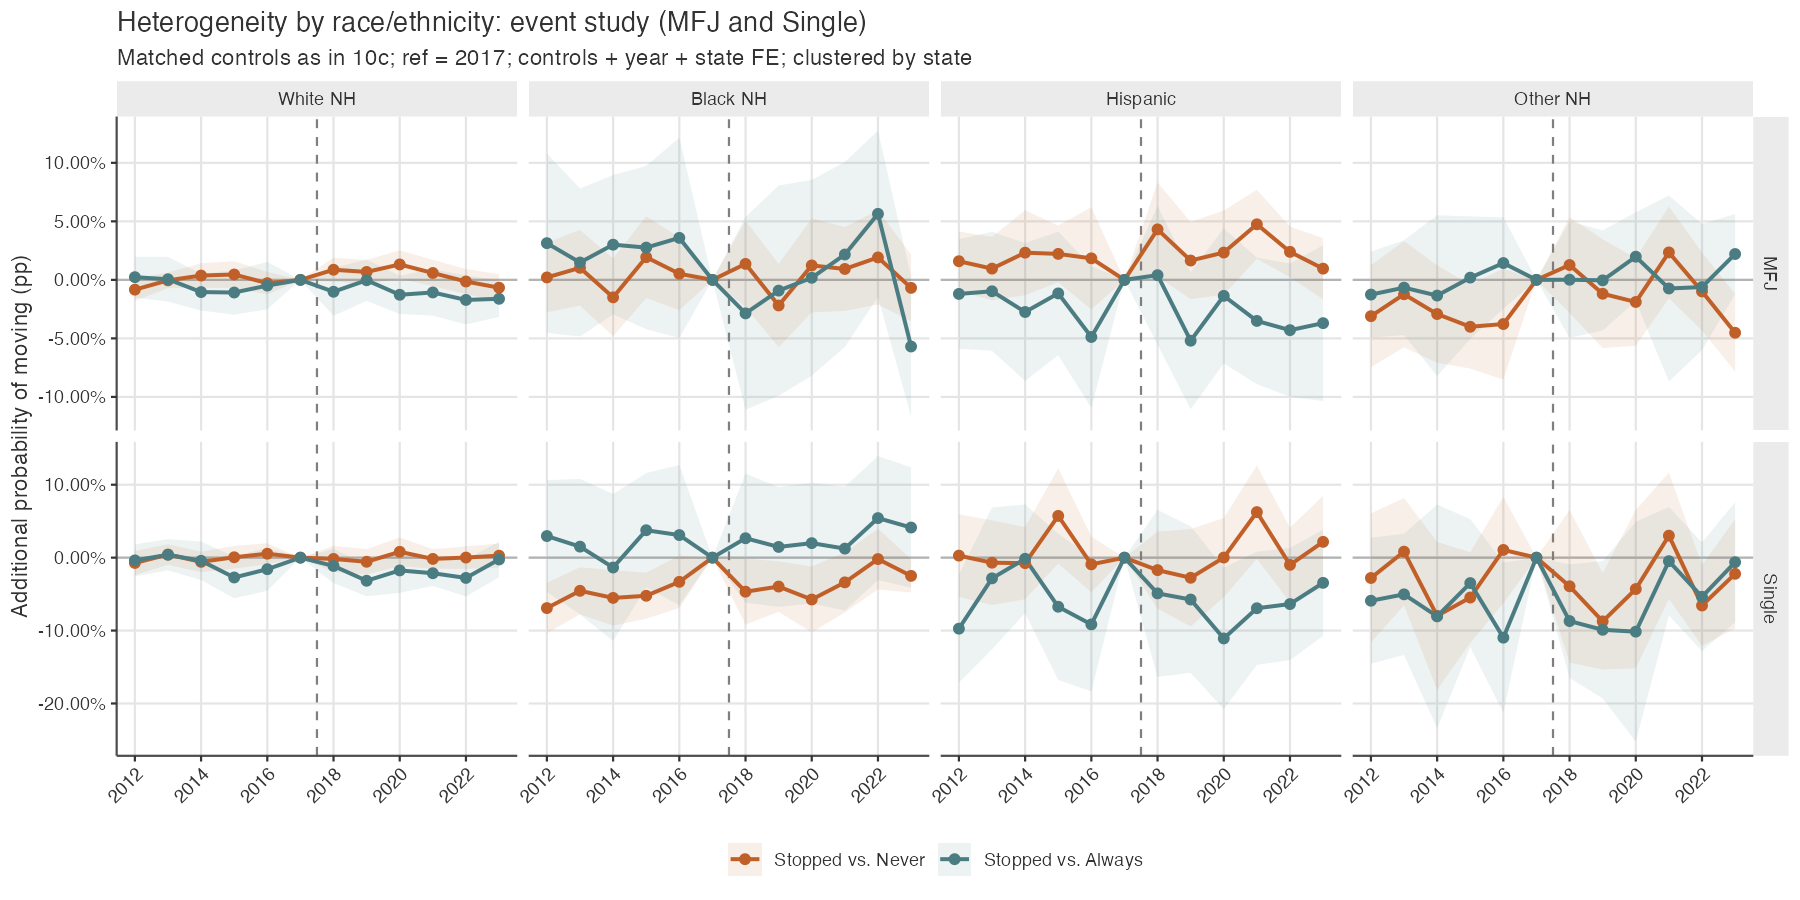
\includegraphics[width=0.7\linewidth]{10d_het_race.png}
\caption{Heterogeneity by race of household head.}
\end{figure}

\begin{figure}[h!]
\centering
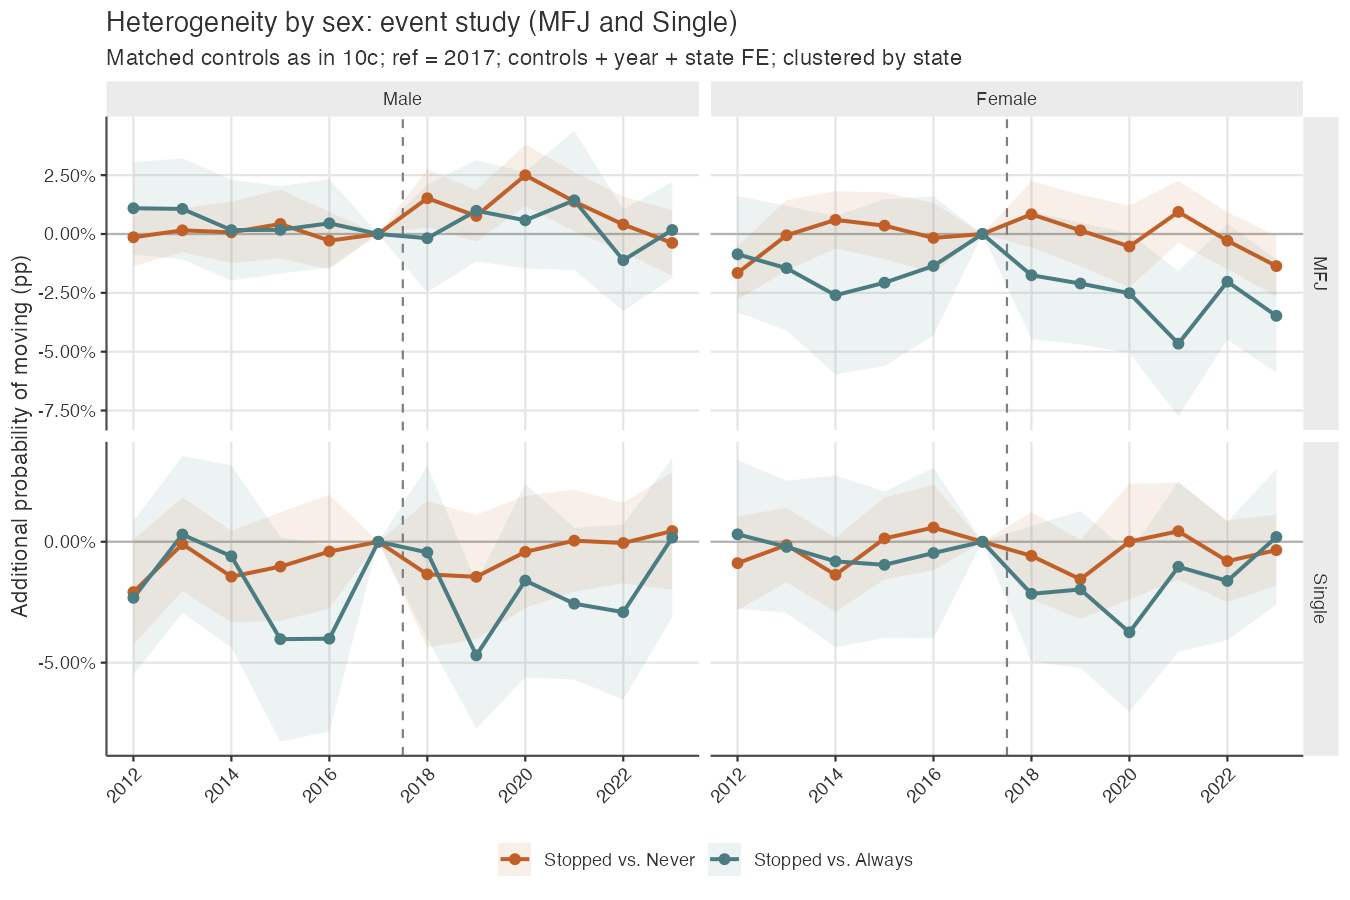
\includegraphics[width=0.7\linewidth]{10d_het_sex.png}
\caption{Heterogeneity by sex of household head.}
\end{figure}

\end{document}
